% !TeX program = xelatex
% HUJOS-TT draft — 19x27cm, Palatino Linotype 10pt, lề 2cm
% NGAN SACH TRANG: HUJOS-TT toi da 12 trang (spec muc 2; ARD mau thuan 12 vs 8-15
% nen giu <= 12 cho ca hai). Cac bien phap NEN khong cat chu: gian dong 1.06,
% caption footnotesize, float/display spacing chat, bang footnotesize, hinh
% 0.84-0.92 textwidth. Tat ca la trinh bay, KHONG xoa noi dung.
% Số liệu: outputs/ (main_raw.csv, wilcoxon_results.csv, sweep_sigma_delta_raw.csv, sweep_salinity_raw.csv)
\documentclass[10pt]{article}
\usepackage[paperwidth=19cm,paperheight=27cm,margin=2cm]{geometry}
\usepackage{fontspec}
% Palatino Linotype là font Windows (không có trên máy Linux build này).
% Build nháp: ưu tiên Palatino Linotype -> Charis SIL (serif họ Palatino, đủ
% dấu tiếng Việt, SIL) -> TeX Gyre Pagella. Bản Word cuối (việc 7) set
% Palatino Linotype thật vì Word của anh có font.
\IfFontExistsTF{Palatino Linotype}{%
  \setmainfont{Palatino Linotype}%
}{%
  \IfFontExistsTF{Charis SIL}{%
    \setmainfont{Charis SIL}%
  }{%
    \setmainfont{TeX Gyre Pagella}%
  }%
}
\setsansfont{DejaVu Sans}
\usepackage{setspace}
\setstretch{1.02}
\usepackage{booktabs}
\usepackage{tabularx}
\usepackage{amsmath,amssymb}
\usepackage{amsthm}
\newtheorem{theorem}{Định lý}
\newtheorem{corollary}{Hệ quả}[theorem]
\newtheorem{proposition}{Mệnh đề}[theorem]
\renewcommand{\proofname}{Chứng minh}
\usepackage{graphicx}
\graphicspath{{../figures/}}
\usepackage[font=footnotesize,labelfont=bf,skip=3pt,labelsep=period]{caption}
% Ten float tieng Viet: PDF sinh 'Bảng 1.' / 'Hình 2.' thay vi 'Table 1:' (sach dau : va het lech ngon ngu).
\captionsetup[table]{name=Bảng}
\captionsetup[figure]{name=Hình}
% NEN KHONG CAT CHU: chat khoang cach doan, float va display de tiet kiem trang.
\setlength{\parskip}{1.5pt plus 1pt minus 0.5pt}
\setlength{\textfloatsep}{6pt plus 2pt minus 2pt}
\setlength{\floatsep}{6pt plus 2pt minus 2pt}
\setlength{\intextsep}{6pt plus 2pt minus 2pt}
\setlength{\abovedisplayskip}{4pt plus 2pt minus 2pt}
\setlength{\belowdisplayskip}{4pt plus 2pt minus 2pt}
\usepackage{titlesec}
\titlespacing{\section}{0pt}{3.5pt}{1.5pt}
\titlespacing{\subsection}{0pt}{3pt}{1pt}
\usepackage[numbers,sort&compress]{natbib}
\renewcommand{\refname}{Tài liệu tham khảo}
\bibliographystyle{unsrtnat}
\usepackage[hidelinks]{hyperref}
\usepackage{enumitem}
\usepackage[ruled,vlined,linesnumbered]{algorithm2e}
\SetAlgorithmName{Thuật toán}{Thuật toán}{Danh sách thuật toán}
% algorithm2e KHONG dung package caption -> labelsep=period khong ap vao no;
% phai doi dau phan cach rieng, neu khong PDF van ra 'Thuật toán 1:'.
\SetAlgoCaptionSeparator{.}
\setlist{nosep,leftmargin=1.2em}
\captionsetup[table]{position=top}
\captionsetup[figure]{position=bottom}

\newcommand{\vn}[1]{#1}

\title{\bfseries Cổng an toàn bản sao số cho phát lệnh tưới trên mạng mất gói và liên hệ với chuẩn MRV phát thải}
\author{}
\date{}

\begin{document}

\maketitle
\vspace{-3em}

{\centering
Mai Xuân Văn\textsuperscript{1}, Nguyễn Tương Tri\textsuperscript{2,3,*}\\
\small \textsuperscript{1}Thuan Hoa High School, University of Education, Hue University\\
\small \textsuperscript{2}University of Education, Hue University, 34 Le Loi St., Hue, Vietnam\\
\small \textsuperscript{3}Institute of Open Education and Information Technology, Hue University\\
\small \textsuperscript{*}Corresponding author: nguyentuongtri@dhsphue.edu.vn\\[6pt]
}

\section*{Tóm tắt}

Chi phí đo đạc, báo cáo và thẩm định (MRV) là nút thắt của tín chỉ các-bon lúa ở Đồng bằng sông Cửu Long; mọi hành vi quản lý nước đủ điều kiện tín chỉ đều đi qua một lệnh điều khiển trên kênh vô tuyến không tin cậy. Chúng tôi đặt bài toán trong khung hệ điều khiển qua mạng (networked control system): một cổng an toàn dùng bản sao số (digital twin) cân bằng nước FAO-56 mô phỏng lệnh ứng viên trước khi gửi, chỉ phát khi ruộng dự báo còn an toàn với xác suất đủ cao, một ràng buộc cơ hội (chance constraint) cho lịch tưới (irrigation scheduling). Chúng tôi chứng minh bản sao số có ngưỡng độ chính xác tính bằng công thức từ độ rộng vùng an toàn: vượt ngưỡng, cổng không phát được lệnh nào và im lặng là tối ưu. Mô phỏng trên thời tiết ERA5 thật tại ba trạm cho thấy cổng giảm giờ mất an toàn so với mọi mốc cơ sở khi nước khan; kiểm định ghép cặp không ô nào cổng thua có ý nghĩa. Chu kỳ ngập--khô xen kẽ đạt chuẩn tín chỉ chỉ xuất hiện khi bản sao số đạt ngưỡng đó, tăng tần suất cảm biến không bù được. Trong mô hình tình huống mặn theo triều, cổng không bao giờ bơm mặn. Nhật ký lệnh là dữ liệu hoạt động cấp MRV theo QĐ 4801/QĐ-BNNMT; mã nguồn công bố tại \url{https://github.com/mxuanvan02/TwinGate}.

\noindent\textbf{Từ khóa:} digital twin; networked control system; chance constraint; irrigation scheduling; MRV

\section{Giới thiệu}

Chương trình một triệu héc-ta lúa chất lượng cao, phát thải thấp vùng Đồng bằng sông Cửu Long (ĐBSCL) theo Quyết định 1490/QĐ-TTg đã vượt mục tiêu giai đoạn đầu với hơn 354\,000 ha vào cuối 2025, nhưng Viện Nghiên cứu Lúa gạo Quốc tế (IRRI) xác định nút thắt tiếp theo không nằm ở kỹ thuật canh tác mà ở chi phí MRV: ``không có hệ thống MRV vận hành được, mức giảm phát thải (dù thật ở cấp ruộng) không thể được chính thức hóa'' thành tài sản tài chính~\cite{irri2026mrv,qd1490}. Quy trình MRV thí điểm của Bộ Nông nghiệp và Môi trường (BNNMT; Quyết định 4801/QĐ-BNNMT ngày 14/11/2025) yêu cầu ``giám sát rút nước trong mùa vụ bằng ảnh chụp và dữ liệu số'' và xếp ``hồ sơ tưới tiêu \& rút nước thực tế'' ở bậc cao nhất trong thứ tự ưu tiên bằng chứng~\cite{qd4801}. Phương pháp luận VM0051 phiên bản 1.1 của Verra, tổ chức vận hành Tiêu chuẩn Các-bon Tự nguyện (VCS), có hiệu lực từ 14/07/2026, khuyến nghị công cụ MRV số (DMRV) cho khâu thẩm định và kiểm chứng (validation/verification), đồng thời bắt buộc nguyên tắc bảo thủ khi chọn tham số~\cite{vm0051}.

Điểm chung của ba văn bản: bằng chứng MRV của quản lý nước ruộng lúa, xét đến cùng, là \emph{bản ghi của các hành động điều khiển nước} (khi nào mở cống, tưới bao nhiêu, có tưới lại hay không) trên các thửa ruộng nhỏ do mạng thiết bị giá rẻ, mất gói vận hành. Trong ngôn ngữ điều khiển qua mạng (NCS), tài nguyên khan hiếm ở đây không phải mẫu cảm biến trên đường truyền lên (uplink) mà là \emph{lệnh điều khiển trên đường truyền xuống} (downlink command). Hai công bố gần đây của chúng tôi, gồm RABS (lập lịch thăm dò an toàn theo rủi ro) và CAW-VoU (đồng bộ bản sao số theo giá trị của thông tin cập nhật), đều đặt dữ liệu uplink làm đối tượng khan hiếm; các nhánh quốc tế về tuổi thông tin (AoI, age of information) và đồng bộ bản sao số (DT-sync) cũng vậy~\cite{rabs,cawvou}. Một khảo sát 461 bản ghi trên cơ sở dữ liệu học thuật mở OpenAlex giai đoạn 2015--2026 cho thấy các nhánh bản sao số, MRV và tín chỉ các-bon, khí mê-tan (CH$_4$) ruộng lúa, tưới ngập--khô xen kẽ (AWD, alternate wetting and drying), và vạn vật kết nối Internet (IoT) trên kênh mất gói đều có mật độ công bố cao, nhưng giao của chúng bằng 0 và chỉ 2/461 công trình đề cập chặn trên bất định hoặc bảo đảm xác suất cho dữ liệu giám sát (chi tiết khảo sát ở Phụ lục~A).

Bài báo này đổi trục nhìn. Thứ khan hiếm không còn là số đo từ ruộng gửi lên mà là lệnh điều khiển gửi xuống ruộng. Bản sao số cũng đổi vai trò: thay vì ước lượng ruộng đang thế nào, nó đứng trước máy phát và trả lời câu hỏi ``nếu gửi lệnh tưới này thì mấy giờ nữa ruộng sẽ ra sao''. Lệnh chỉ được gửi khi câu trả lời đủ an toàn. Bài báo có ba đóng góp:

\begin{enumerate}
\item \textbf{Một cơ chế cổng an toàn cho lệnh tưới} trên kênh mất gói theo cụm~\cite{gilbert1960,elliott1963}. Hệ thống quyết định mỗi ngày một lần, khớp nhịp vận hành cống và bơm ngoài thực tế; nước có hạn mức cho cả mùa vụ; và im lặng là một lựa chọn hợp lệ chứ không phải sự cố.
\item \textbf{Một ngưỡng cho độ chính xác của bản sao số} (Định lý 1 và Hệ quả 1). Mức an toàn mà hệ thống hứa được quyết định bởi tương quan giữa độ rộng vùng an toàn nông học và độ mờ của bản sao số. Khi bản sao mờ quá ngưỡng, cổng không còn lệnh nào để phát, bất kể thiết bị chấp hành có những mức tưới nào. Chúng tôi kiểm chứng bằng cách quét đồng thời hai tham số và thu được đúng mặt ngưỡng mà lý thuyết dự đoán.
\item \textbf{Một khung mô phỏng chạy lại được từ đầu} trên dữ liệu tái phân tích khí quyển ERA5 của Trung tâm Dự báo Thời tiết Hạn vừa châu Âu (ECMWF), tại ba trạm ĐBSCL, trong hai năm khí hậu trái ngược nhau (2024 khan nước, 2025 dư nước), kèm một mô hình \emph{tình huống} nước mặn theo triều để lượng hóa cái giá của việc chờ con nước.
\end{enumerate}

\section{Công trình liên quan}

\emph{Tuổi thông tin và đồng bộ bản sao số.} Nhánh nghiên cứu về tuổi thông tin (AoI) tối ưu độ tươi mới của luồng dữ liệu trên đường uplink; các bộ lập lịch trong nhánh này luôn phải phát một gói nào đó và không có khái niệm ``cổng rỗng''. So sánh theo trục (tài nguyên khan hiếm, vai trò twin, ràng buộc an toàn) với RABS và CAW-VoU~\cite{rabs,cawvou} được tóm tắt ở Bảng~\ref{tab:gap}.

\emph{AWD và MRV lúa.} Tưới ngập--khô xen kẽ (AWD) giảm CH$_4$ 48--93\% và giảm nước 23--33\%~\cite{balaine2019,carrijo2017,yan2005}; rào cản nhân rộng là thể chế và đo lường chứ không phải kỹ thuật~\cite{enriquez2021,lampayan2015}. Giám sát AWD hiện dựa vào ống quan trắc thủ công, cảm biến mực nước không dây giá rẻ~\cite{delacruz2022}, viễn thám bằng vệ tinh radar ALOS-2 của Nhật Bản~\cite{islam2026alose}, hoặc phân loại thực hành bằng viễn thám quy mô vùng~\cite{lovell2019,mlrice2025}; chưa công trình nào định lượng độ tin cậy của bản ghi hành động khi mạng mất gói.

\emph{Điều khiển an toàn với thông tin không hoàn hảo.} Các phương pháp điều khiển với ràng buộc cơ hội (chance-constrained control) và hàm rào cản điều khiển (control barrier function) giả định trạng thái đo được hoặc ước lượng được với một chặn trên bất định đã biết; ở đây chính chặn trên đó ($\sigma$ của bản sao số, tăng theo tuổi dữ liệu) trở thành tham số của bảo đảm an toàn và có ngưỡng chết $\sigma^{*}$, một dạng ``ngân sách độ trung thực'' (fidelity budget) mà chúng tôi không tìm thấy trong văn liệu đồng bộ bản sao số (Phụ lục~A).

\begin{table}[h]
\centering
\caption{Vị trí bài báo so với các nhánh liên quan}
\label{tab:gap}
\footnotesize
\begin{tabularx}{\textwidth}{@{}>{\raggedright}p{2.4cm} >{\raggedright\arraybackslash}X >{\raggedright\arraybackslash}X >{\raggedright\arraybackslash}X >{\raggedright\arraybackslash}X@{}}
\toprule
Trục so sánh & Các nhánh tuổi thông tin và đồng bộ bản sao số & RABS~\cite{rabs} & CAW-VoU~\cite{cawvou} & Bài báo này \\
\midrule
Tài nguyên khan hiếm & gói dữ liệu trên đường uplink & ngân sách thăm dò (polling) & khe dò (probe slot) & \textbf{lệnh trên đường downlink} \\
Vai trò của bản sao số & bản sao trạng thái & bộ dự báo Kalman & bộ dự báo & \textbf{cổng nhận $u$ làm đầu vào để trả lời câu hỏi phản thực} \\
Ràng buộc an toàn & không có & ngưỡng tĩnh & ngưỡng tĩnh, xét tại một thời điểm & \textbf{ràng buộc cơ hội kèm ngưỡng $\sigma^{*}$} \\
Hành động ``không phát'' & không tồn tại & không tồn tại & không tồn tại & \textbf{WITHHELD là tối ưu} \\
Mối nguy thứ hai & không & không & không & \textbf{độ mặn nguồn nước biến thiên theo triều (mô hình tình huống)} \\
\bottomrule
\end{tabularx}
\end{table}

\section{Mô hình hệ thống}

\subsection{Ruộng, twin và tập an toàn}

Trạng thái ruộng là lượng nước tầng rễ $w$ [mm], mô hình hóa theo cân bằng nước ``bể chứa'' (bucket) của Tài liệu hướng dẫn tưới tiêu và thoát nước số 56 do Tổ chức Lương thực và Nông nghiệp Liên Hợp Quốc ban hành, gọi tắt là FAO-56~\cite{fao56}. Mỗi giờ, $w$ nhận mưa (sau khi trừ dòng chảy mặt tính bằng phương pháp đường cong số hiệu SCS-CN của Cục Bảo tồn Đất đai Hoa Kỳ, tính ở độ phân giải ngày rồi chia theo tỷ lệ cho từng giờ mưa) và nước tưới; mất đi do bốc thoát hơi nước cây trồng $ET_c = K_s K_c ET_0$, trong đó $ET_0$ là bốc thoát hơi nước tham chiếu tính theo công thức Penman--Monteith dạng giờ (vận tốc gió quy đổi từ độ cao 10\,m về 2\,m theo phương trình 47 của FAO-56), $K_c$ là hệ số cây trồng và $K_s$ là hệ số giảm do stress nước; và tiêu thoát phần vượt quá dung trọng đồng ruộng. Định luật bảo toàn khối lượng được kiểm chứng bằng một bất biến với phần dư (residual) đúng bằng 0. Đất lấy theo loại thịt pha sét (silty-clay loam) điển hình của ĐBSCL với tham số trung bình ở Bảng 2 của FAO-56, tầng rễ 0,5\,m, suy ra tổng lượng nước hữu hiệu TAW (total available water) $= 70$\,mm, dung trọng đồng ruộng FC (field capacity) $= 160$\,mm và điểm héo WP (wilting point) $= 90$\,mm.

Tập an toàn nông học $S = [w_{lo}, w_{hi}]$ tương ứng với độ cạn kiệt (depletion fraction) trong khoảng $[0; 0{,}85]$, suy ra chiều rộng tập an toàn $W = w_{hi} - w_{lo} = 59{,}5$\,mm. Twin $\hat w$ tiến hóa theo cùng thời tiết nhưng theo lượng nước gateway \emph{tin rằng} đã tới ruộng, được tái neo (re-anchor) bởi số đo cảm biến trên đường uplink với xác suất mất gói $p_{ul}=0{,}15$. Độ bất định dự báo của bản sao số tăng theo tuổi $a$ (số giờ kể từ lần tái neo gần nhất) theo luật phương sai của mô hình tự hồi quy bậc một AR(1) và bộ lọc Kalman, kế thừa từ~\cite{cawvou}:
\begin{equation}
\sigma(a) \;=\; \min\!\Big(\sigma_0 \sqrt{\textstyle\sum_{k=0}^{a} \rho^{2k}},\ \ \sigma_0/\sqrt{1-\rho^2}\Big),\qquad \sigma_0 = f_\sigma \cdot \mathrm{TAW},\ \rho=0{,}9,
\label{eq:sigma}
\end{equation}
trong đó $f_\sigma$ là tham số độ trung thực duy nhất, biểu thị độ lệch chuẩn dự báo của bản sao số theo tỷ lệ trên TAW.

\subsection{Kênh lệnh và epoch quyết định}

Đường downlink được mô hình hóa bằng kênh Gilbert--Elliott hai trạng thái (tốt/xấu, mất gói theo cụm)~\cite{gilbert1960,elliott1963} với hai cấu hình ``mild'' (mất gói nhẹ) và ``severe'' (mất gói nặng) nêu ở Bảng~\ref{tab:setup}. Tín hiệu xác nhận ACK (acknowledgement) gửi ngược về bị mất với xác suất 0,35, nên việc ``không nhận được ACK'' thực sự mơ hồ: lệnh có thể đã mất, hoặc lệnh đã tới ruộng nhưng ACK bị mất. Cổng (gateway) duy trì niềm tin $\pi_k = 1-(1-\varphi)^k$ với $\varphi = p_{dl}(1-p_{ack})$ rằng lệnh đang chờ đã tới ruộng, trong đó $k$ là số lần gửi và $p_{dl}$, $p_{ack}$ lần lượt là xác suất thành công của đường downlink và của ACK. Chính sách gửi lại mà chúng tôi đề xuất, ký hiệu \textbf{T2}, gửi lại khi và chỉ khi $\pi$ thấp hơn một ngưỡng tối ưu cận biên (myopic) của chi phí kỳ vọng, đánh đổi giữa hai rủi ro là tưới đúp và mất lệnh. Mỗi lệnh mang một độ sâu tưới lấy từ tập ứng viên nông học $\{20, 40, 60\}$\,mm. Hệ thống chỉ ra \textbf{một quyết định mỗi chu kỳ (epoch) 24 giờ}, trong đó quyết định im lặng (WITHHELD) cũng tiêu tốn chu kỳ đó, nhằm khớp với nhịp vận hành cống và bơm ngoài thực tế. Nếu bỏ giới hạn này thì bộ chỉ số mất khả năng phân biệt: với tập ứng viên mịn $0$--$30$\,mm và không có ràng buộc ngân sách, chúng tôi đo được cả ba chính sách đều đạt $0\%$ giờ mất an toàn nên không còn gì để so sánh; với tập ứng viên nông học hiện tại, bỏ trần chu kỳ làm giờ mất an toàn tăng thêm $1{,}96$ điểm ở dải $f_\sigma=0{,}02$ (kênh severe, các ngân sách ràng buộc). Cả hai phép đo đều tái lập được từ mã nguồn công bố.

\subsection{Ngân sách nước và các chính sách so sánh}

Ngân sách nước mùa vụ $B$ (tính bằng mm nước \emph{đã thực sự tới ruộng}) là ràng buộc cứng áp cho cả lệnh mới lẫn lệnh gửi lại, nên không chính sách nào có thể vượt ngân sách (bất biến I1 ghi nhận mức vượt tệ nhất là 0,000\,mm trên 108 lần mô phỏng). Bảy chính sách được so sánh: (i) \textbf{TwinGate+T2} là chính sách đề xuất, gồm cổng bản sao số, luật chọn lệnh thích ứng và cơ chế gửi lại T2; (i$'$) TwinGate+T2+centre là \emph{đối chứng của riêng luật chọn lệnh}, giống hệt chính sách đề xuất nhưng luôn chọn lệnh đưa trạng thái về giữa tập an toàn thay vì về biên khô khi nước khan; (ii) TwinGate+blindARQ giữ cổng nhưng gửi lại mù, tức là gửi lại mọi lần thiếu ACK mà không xét niềm tin (ARQ viết tắt của \emph{automatic repeat request}); (iii) Reactive+T2 thay cổng bằng một ngưỡng độ cạn kiệt tĩnh 0,55 và vẫn gửi lại theo niềm tin; (iv) Reactive+blindARQ kết hợp ngưỡng tĩnh với gửi lại mù; (v) FixedSchedule mô phỏng tập quán canh tác, tưới cố định 60\,mm mỗi năm ngày theo lịch mà không quan sát ruộng; và (vi) \textbf{Oracle} là bộ điều khiển tối ưu với thông tin hoàn hảo, thấy trạng thái thật $w_{true}$ và khôi phục về độ cạn kiệt 0,80 bằng độ sâu nhỏ nhất đủ, đóng vai trò mốc tham chiếu về khả năng đạt được.

\subsection{Cổng an toàn (cơ chế đề xuất)}

Hình~\ref{fig:method} trình bày toàn bộ luồng dữ liệu và ba kết cục của một chu kỳ quyết định; Thuật toán~\ref{alg:gate} mô tả chi tiết từng bước.

\begin{figure}[t]
\centering
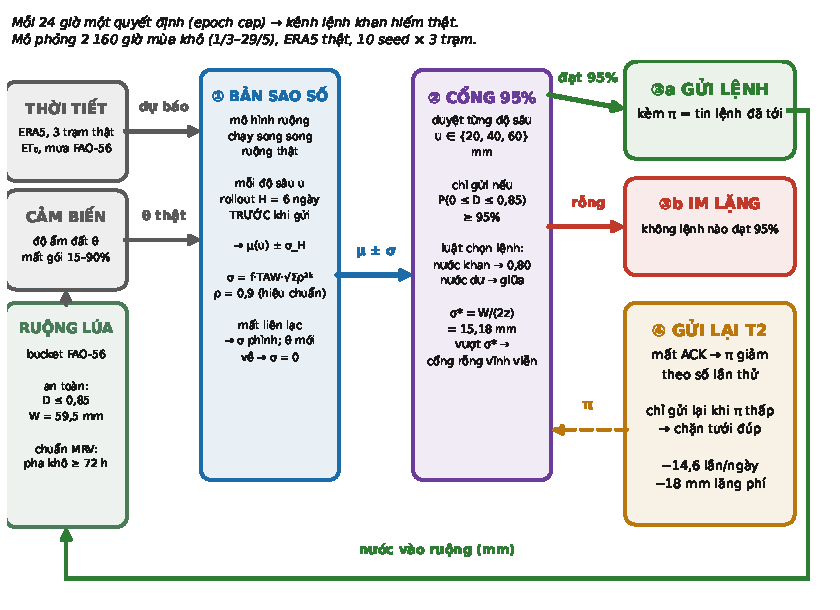
\includegraphics[width=\textwidth]{fig1_method.pdf}
\caption{Cơ chế đề xuất. Bản sao số FAO-56 trả lời câu hỏi phản thực ``nếu phát độ sâu $u$ thì ruộng ở đâu sau $H$ giờ''; cổng chỉ phát lệnh khi xác suất trạng thái sau lệnh nằm trong tập an toàn đạt $1-\delta$. Ba kết cục của một chu kỳ: phát lệnh (kèm niềm tin $\pi$), im lặng (WITHHELD) khi không lệnh nào đạt ngưỡng, và gửi lại T2 khi $\pi$ còn thấp. Mỗi 24 giờ một quyết định nên kênh lệnh khan hiếm thật.}
\label{fig:method}
\end{figure}

Toàn bộ cơ chế đề xuất trong một chu kỳ quyết định được tóm tắt ở Thuật toán~\ref{alg:gate}. Ba điểm làm nên khác biệt so với bộ lập lịch thông thường: (a) lệnh được \emph{mô phỏng trước khi gửi} nhờ bản sao số nhận $u$ làm đầu vào; (b) im lặng là một kết quả hợp lệ của thuật toán, không phải ngoại lệ; và (c) việc gửi lại được điều khiển bởi niềm tin $\pi$ chứ không gửi mù.

\begin{algorithm}[t]
\caption{Cổng an toàn + gửi lại T2 trong một chu kỳ quyết định (24 giờ)}
\label{alg:gate}
\KwIn{niềm tin trạng thái $\hat w$, tuổi dữ liệu $a$, ngân sách còn lại $B_{rem}$, tập ứng viên $\mathcal{U}=\{0;20;40;60\}$\,mm, tham số $\delta$, $H$, $f_\sigma$}
\KwOut{phát một lệnh $u^{*}>0$, hoặc WITHHELD kèm lý do}
$\mathcal{U}_{aff} \leftarrow \{u \in \mathcal{U} : u \le B_{rem}\}$\;
\If{đã bật ràng buộc mặn theo triều (ký hiệu C2, trình bày ở Mục~\ref{sec:salinity}) và giờ hiện tại nguồn không đủ ngọt}{
  \If{còn giờ ngọt nào trong chu kỳ}{\Return{chờ tới giờ ngọt (không tiêu chu kỳ)}}
  \Return{WITHHELD, lý do nguồn mặn, không có ``con nước''}
}
\ForEach{$u \in \mathcal{U}_{aff}$}{
  $(\mu(u), \sigma_H) \leftarrow$ mô phỏng tiến bản sao số $H$ giờ với $u$ áp vào giờ đầu; $\sigma_H = \sigma(a+H)$ theo~\eqref{eq:sigma}\;
  $p(u) \leftarrow \Phi\big(\tfrac{w_{hi}-\mu(u)}{\sigma_H}\big) - \Phi\big(\tfrac{w_{lo}-\mu(u)}{\sigma_H}\big)$\;
}
$\mathcal{P} \leftarrow \{u \in \mathcal{U}_{aff} : p(u) \ge 1-\delta,\ u>0\}$\;
\If{$\mathcal{P} = \emptyset$}{\Return{WITHHELD, lý do: ràng buộc cơ hội không đạt (kể cả khi $\sigma_H \ge \sigma^{*}$)}}
$d^{*} \leftarrow 0{,}80$ \If{$B_{rem} \ge D_{\mathrm{con}}$}{ $d^{*} \leftarrow (w_{hi}+w_{lo})/2$ }\;
$u^{*} \leftarrow \arg\min_{u \in \mathcal{P}} \big|\mu(u) - (\mathrm{FC} - d^{*}\cdot \mathrm{span})\big|$\;
gửi $u^{*}$ qua downlink; $k \leftarrow 1$\;
\While{không nhận được ACK và $\pi_k < \pi^{\dagger}$ và $u^{*} \le B_{rem}$}{
  $\pi_k \leftarrow 1-(1-\varphi)^k$ \tcp*{niềm tin lệnh đã tới ruộng}
  gửi lại $u^{*}$; $k \leftarrow k+1$ \tcp*{chính sách T2}
}
\end{algorithm}

Với lệnh ứng viên $u$, bản sao số được mô phỏng tiến (rollout) $H=6$ giờ với $u$ áp vào giờ đầu tiên:
\begin{equation}
\mu(u) = \mathbb{E}\big[w_{t+H} \mid \hat w_t, u\big], \qquad
p(u) = \Phi\!\Big(\tfrac{w_{hi}-\mu(u)}{\sigma_H}\Big) - \Phi\!\Big(\tfrac{w_{lo}-\mu(u)}{\sigma_H}\Big),
\label{eq:gate}
\end{equation}
với $\sigma_H = \sigma(a+H)$ theo~\eqref{eq:sigma}. Cổng phát $u$ chỉ khi $p(u) \ge 1-\delta$. Trong các lệnh đạt, \emph{luật chọn lệnh thích ứng} quyết định đích đến: gọi $D_{\mathrm{con}}$ là thiếu hụt nước dự báo của phần mùa còn lại (tính bằng chính chuỗi thời tiết mà bản sao số dùng, nên không thêm tham số tự do nào), nếu $B_{rem} < D_{\mathrm{con}}$ thì chọn lệnh đưa $\mu(u)$ về độ cạn kiệt $d^{*}=0{,}80$, sát biên khô để kéo dài ngân sách; ngược lại chọn lệnh về giữa tập an toàn để tối đa biên an toàn. Lệnh 0\,mm không được truyền vì truyền 0\,mm vẫn tốn một lần dùng kênh và làm sai các chỉ số đo (metric) về lượng nước mỗi lệnh. Nếu không lệnh nào đạt: WITHHELD.

\section{Lý thuyết}

\begin{theorem}[Soundness của cổng]
\label{thm:t1}
Nếu phần dư (residual) của bản sao số có phân phối chuẩn (Gaussian) với độ lệch chuẩn $\sigma_H$ tại chân trời $H$, thì mọi lệnh được cổng~\eqref{eq:gate} giải phóng đều thỏa mãn $P\big(w_{t+H} \in S\big) \ge 1-\delta$.
\end{theorem}
\begin{proof}
Điều kiện lọc của cổng chính là $p(u)\ge 1-\delta$ với $p(u)$ là xác suất Gaussian của~\eqref{eq:gate}.
\end{proof}

\begin{corollary}[Ngưỡng độ trung thực $\sigma^{*}$]
\label{cor:sigma}
Tồn tại lệnh được phát chỉ khi $\exists u:\ \mu(u) \in \big[w_{lo} + z_{1-\delta/2}\sigma_H,\ w_{hi} - z_{1-\delta/2}\sigma_H\big]$. Điều kiện cần, độc lập tập lệnh:
\begin{equation}
\sigma_H < \sigma^{*} \;\equiv\; \frac{W}{2\,z_{1-\delta/2}} .
\label{eq:sigmastar}
\end{equation}
Khi $\sigma_H \ge \sigma^{*}$, cổng \emph{rỗng với mọi tập lệnh} và WITHHELD là hành vi đúng duy nhất.
\end{corollary}

Với $W = 59{,}5$\,mm: $\sigma^{*} = 44{,}11$\,mm ($\delta{=}0{,}5$); 23,21\,mm ($\delta{=}0{,}2$); \textbf{15,18\,mm} ($\delta{=}0{,}05$); 11,55\,mm ($\delta{=}0{,}01$). Về mặt khoa học, $\delta$ và $\sigma$ không độc lập vì mọi bảo đảm an toàn đều đi qua tỉ số $W/\sigma_H$, một đại lượng \emph{đo được} của cặp (độ rộng vùng an toàn nông học, độ trung thực của bản sao số). Dự đoán của~\eqref{eq:sigmastar} được kiểm bằng số ở Mục~\ref{sec:sweep} và bằng bất biến I6 ở Mục~\ref{sec:invariants}.



\begin{proposition}[Số lệnh phân biệt được, và khi nào luật chọn lệnh trở nên vô hiệu]
\label{prop:dmax}
Gọi $\mathcal{U}$ là tập độ sâu ứng viên, $\Delta_{\min}$ là bước nhảy nhỏ nhất giữa hai phần tử kề nhau của $\mathcal{U}$, và $z=z_{1-\delta}$. Với một niềm tin cố định, tập lệnh đạt yêu cầu
\[
\mathcal{P} \;=\; \big\{u\in\mathcal{U}:\ \mu(u) \in [\,w_{lo}+z\sigma_H,\ w_{hi}-z\sigma_H\,]\big\}
\]
nằm trong một khoảng có độ dài $W-2z\sigma_H$. Do đó
\begin{equation}
|\mathcal{P}| \;\le\; 1 + \frac{|W-2z\sigma_H|}{\Delta_{\min}},
\label{eq:dmax}
\end{equation}
và hệ quả trực tiếp: nếu $W-2z\sigma_H < \Delta_{\min}$ thì tại \emph{mỗi} niềm tin chỉ có nhiều nhất một ứng viên đạt yêu cầu, nên \emph{mọi} luật chọn lệnh (về giữa tập an toàn, về biên khô, hay bất kỳ luật nào khác) đều trả về cùng một lệnh.
\end{proposition}
\begin{proof}
Bất đẳng thức \eqref{eq:dmax} là đếm số điểm của một lưới có bước $\Delta_{\min}$ rơi vào một khoảng. Phần ``hệ quả'' suy ra từ $|\mathcal{P}|\le 1$. Lưu ý bất đẳng thức chỉ là \emph{chặn trên}; nó không khẳng định $\mathcal{P}\neq\emptyset$ (điều kiện đó là Hệ quả~\ref{cor:sigma}) và cũng không khẳng định hai ứng viên kề nhau luôn cho $\mu$ cách nhau đúng $\Delta_{\min}$, vì phép cuộn (rollout) là phi tuyến do bucket bị chặn ở dung trọng đồng ruộng, nên hai độ sâu khác nhau có thể cho cùng $\mu$.
\end{proof}

Với $W=59{,}5$\,mm, $\Delta_{\min}=20$\,mm và $\delta=0{,}05$, Mệnh đề~\ref{prop:dmax} dự đoán vùng đạt yêu cầu rộng $59{,}5-2(1{,}96)\sigma_H$, tức hẹp hơn 20\,mm khi $\sigma_H>10{,}08$\,mm, tương ứng $f_\sigma>0{,}0715$. Dự đoán này được kiểm bằng số ở Mục~\ref{sec:sweep}: tại $f_\sigma=0{,}10$ ($\sigma_H=14{,}1$\,mm) hai luật chọn lệnh cho kết quả \emph{giống hệt nhau} ở 36/36 ô, trong khi tại $f_\sigma=0{,}02$ (vùng đạt yêu cầu rộng 48,4\,mm) chúng khác nhau ở 18/36 ô với ý nghĩa thống kê. Kiểm chứng mạnh hơn là đếm trực tiếp số ứng viên lọt vào vùng đạt yêu cầu trên lưới belief: đo được 3 ứng viên khi lý thuyết dự đoán 3, 2 khi dự đoán 2, và 1 khi dự đoán 1, với bước nhảy thực của $\mu$ đo được là 15,35\,mm.

Một hệ quả thực tế quan trọng: vì $\sigma_H$ có \emph{giới hạn dưới} $f_\sigma\cdot\mathrm{TAW}\cdot g$ ngay cả khi tuổi dữ liệu bằng 0 (tức vừa được tái neo), nên \textbf{tăng tần suất cảm biến không thể cứu một bản sao số thô}. Với $f_\sigma=0{,}10$, giới hạn dưới đó là 14,10\,mm, lớn hơn 3,57\,mm cần cho AWD; ngược lại với $f_\sigma=0{,}02$ thì $\sigma$ tĩnh chỉ 3,21\,mm, nên cổng vẫn làm được AWD \emph{ngay cả khi không bao giờ được tái neo} (pin yếu hoặc kênh nghẽn). Đây là thông tin thiết kế trực tiếp cho việc chọn thiết bị, trình bày ở Mục~\ref{sec:deploy}.

\section{Thiết kế thực nghiệm}

\begin{table}[h]
\centering
\caption{Cấu hình thực nghiệm (mọi số đều tái lập từ mã nguồn)}
\label{tab:setup}
\footnotesize
\begin{tabular}{@{}p{2.9cm}p{11.5cm}@{}}
\toprule
Thành phần & Giá trị \\
\midrule
Thời tiết & ERA5, tải qua giao diện lập trình ứng dụng (API) lưu trữ của Open-Meteo, độ phân giải giờ, 3 trạm: Cần Thơ (10,0452N; 105,7469E), Sóc Trăng (9,6037N; 105,9739E), Cà Mau (9,1769N; 105,1524E); năm 2024 và 2025, không có giá trị khuyết, kèm tệp xuất xứ định dạng JSON \\
Cửa sổ & 1/3--29/5 (2160 giờ): ERA5 đo được ~100\% giờ sốc nhiệt năm rơi vào III--V \\
Thiếu hụt mùa & ròng $K_c\sum ET_0-\sum P$: 302--318\,mm; theo giờ $\sum_h\max(0,K_cET_{0,h}-P_h)$: 450--485\,mm (tùy trạm). Bộ điều khiển xét ``khan'' bằng đại lượng thứ hai (không cho mưa dư bù trừ, là cách làm thận trọng), nên mọi $B$ hữu hạn trong lưới đều ràng buộc \\
Chu kỳ quyết định & 24 giờ; các mức ứng viên độ sâu $\{20;40;60\}$\,mm \\
Downlink & mild: $(p_{gb},p_{bg},\ell_g,\ell_b)=(0{,}06;0{,}22;0{,}035;0{,}65)$; severe: $(0{,}08;0{,}15;0{,}82;0{,}15)$, tham số hóa như~\cite{rabs,cawvou} \\
Uplink / ACK & mất 15\% / 35\% \\
Ngân sách nước $B$ & 80 / 160 / 240 / 320 / 400 / $\infty$ mm \\
Hạt giống ngẫu nhiên & 10 hạt giống (seed)/ô; bộ sinh số ngẫu nhiên (RNG) tách theo vai trò, mọi chính sách nhận cùng một dãy biến cố kênh \\
Lưới thí nghiệm chính & 3 trạm $\times$ 2 kênh $\times$ 6 mức $B$ $\times$ 7 chính sách $\times$ 10 hạt giống $\times$ 3 dải độ trung thực $f_\sigma\in\{0{,}02;\,0{,}05;\,0{,}10\}$ $=$ \textbf{7560} lần mô phỏng mỗi năm \\
Các lưới bổ trợ & ablation 8 biến thể (4800); triển khai 5 yếu tố (540); đa ruộng 6 thửa $\times$ 3 luật phân bổ (2700); quét $f_\sigma\times\delta$ (4320); tình huống mặn (1800) \\
Thống kê & kiểm định Wilcoxon ghép cặp theo dấu hạng, ghép cặp theo hạt giống trong từng ô, hiệu chỉnh Holm trong mỗi ô, cỡ hiệu quả là tương quan hạng hai chiều $r=Z/\sqrt{n}$ \\
\bottomrule
\end{tabular}
\end{table}

\emph{Ba dải độ trung thực.} Độ trung thực $f_\sigma$ không được chọn tùy ý mà suy ra từ hai ngưỡng tính được bằng công thức (Mục~\ref{sec:deploy}): $\sigma^{*}=15{,}18$\,mm là ngưỡng cổng \emph{sống} (phát được ít nhất một lệnh), và $\sigma_H \le 3{,}57$\,mm là ngưỡng để chu kỳ khô kéo dài đủ 72 giờ theo QĐ 4801. Ba mốc quét là $f_\sigma=0{,}02$ (dải \texttt{awd}: đạt cả hai ngưỡng), $0{,}05$ (dải \texttt{mid}: ở giữa) và $0{,}10$ (dải \texttt{narrow}: cổng vẫn sống nhưng AWD không còn khả thi). Việc báo cáo cả ba dải là bắt buộc: một cơ chế chỉ đúng ở một mức độ trung thực tùy ý thì không phải là đóng góp.

\emph{Nguyên tắc chống tự đánh lừa kết quả.} Thứ nhất, mọi chỉ số đo đều có bộ kiểm tra tự động: chỉ số bị bão hòa, tỷ lệ mất an toàn không còn giảm đơn điệu khi ngân sách $B$ tăng, cơ chế T2 không tạo khác biệt so với gửi lại mù, mốc Oracle tệ hơn các mốc cơ sở, hoặc cổng chuyển sang ``tưới nhỏ giọt'' với lượng nước không đủ ý nghĩa nông học; bất kỳ vi phạm nào cũng khiến tập lệnh trả về mã thoát khác không. Thứ hai, bảy bất biến (I1 ngân sách cứng; I2 mỗi chu kỳ một quyết định; I3 không tưới nhỏ giọt; I4 bảo toàn khối lượng; I5 mốc Oracle hợp lệ; I6 hành vi ngưỡng $\sigma^{*}$; I7 hiệu chuẩn dải 95\%) được chạy dưới dạng bộ kiểm thử tự động. Thứ ba, khi một kiểm thử không đạt, chúng tôi tính lại giá trị kỳ vọng bằng tay một cách độc lập trước khi quyết định sửa mã nguồn hay sửa kiểm thử; chính quy trình này đã phát hiện ba lỗi thuộc về bản thân kiểm thử và bộ kiểm tra trong quá trình phát triển.

\section{Kết quả}

\emph{Nguồn số liệu:} mọi bảng và hình trong mục này được \textbf{sinh tự động} từ \texttt{outputs/*.csv} bằng \texttt{experiments/make\_latex\_tables.py} và \texttt{figures/}; không con số nào được nhập tay vào bản thảo, nên mỗi giá trị đều truy ngược được về lần mô phỏng đã sinh ra nó.

\subsection{Đánh đổi giữa an toàn và lượng nước (mùa khô 2024, điều kiện khan hiếm)}
\label{sec:tradeoff}

Bảng~\ref{tab:main2024} trình bày tỷ lệ giờ mất an toàn ở dải độ trung thực cao nhất ($f_\sigma=0{,}02$), trung bình trên 30 lần mô phỏng mỗi ô. Với $B$ có hiệu lực, tức ngân sách thực sự ràng buộc quyết định, TwinGate+T2 thấp hơn mọi mốc cơ sở tại mọi ô: 34,79\% so với 41,27--53,78\% ở $B{=}80$, và 0,81\% so với 11,30--48,39\% ở $B{=}240$. Khoảng cách tới mốc Oracle (31,92\% ở $B{=}80$; 0,01\% ở $B{=}240$) là ``giá của thông tin không hoàn hảo''. FixedSchedule, tập quán tưới theo lịch mà không quan sát ruộng, tệ nhất ở mọi mức ràng buộc, đúng thông điệp vận hành: lịch cố định dưới ràng buộc nước là chiến lược bị chi phối. Hình~\ref{fig:pareto} vẽ toàn bộ mặt đánh đổi này cho cả bảy chính sách trên ba dải độ trung thực.

\begin{table}[t]
\centering
\caption{Tỷ lệ giờ mất an toàn (\%) theo ngân sách nước mùa vụ, trung bình ba trạm, mùa khô 2024, kênh mất gói nặng (severe), dải $f_\sigma=0{,}02$. Ở kênh mild sai khác dưới 0,2 điểm phần trăm. Ngân sách ràng buộc: \emph{mọi} mức hữu hạn 80--400\,mm trong lưới đều nhỏ hơn thiếu hụt mùa mà chính bộ điều khiển dùng để xét khan ($\sum_h\max(0, K_cET_{0,h}-P_h) = 450$--$485$\,mm tùy trạm), nên đều ràng buộc; chỉ $B=\infty$ là không. Thiếu hụt ròng vật lý $K_c\sum ET_0-\sum P$ là 302--318\,mm; hai đại lượng này khác nhau vì cách thứ nhất không cho mưa dư bù trừ. Bảng đầy đủ cho cả ba dải và hai kênh: \texttt{outputs/main\_summary.csv}.}
\label{tab:main2024}
\footnotesize
\begin{tabular}{@{}lrrrrrr@{}}
\toprule
Chính sách & $B{=}80$ & $B{=}160$ & $B{=}240$ & $B{=}320$ & $B{=}400$ & $B{=}\infty$ \\
\midrule
\textbf{TwinGate+T2} & \textbf{34,79} & \textbf{14,47} & \textbf{0,81} & 0,26 & 0,10 & 0,02 \\
TwinGate+T2+centre & 41,27 & 25,87 & 11,30 & \textbf{0,04} & \textbf{0,02} & \textbf{0,02} \\
TwinGate+blindARQ & 36,36 & 17,45 & 2,48 & \textbf{0,00} & \textbf{0,00} & \textbf{0,00} \\
Reactive+T2 & 45,52 & 34,85 & 28,10 & 17,82 & 7,36 & 0,02 \\
Reactive+blindARQ & 46,55 & 36,61 & 36,22 & 25,65 & 16,78 & 0,00 \\
FixedSchedule & 53,78 & 47,98 & 48,39 & 39,07 & 32,23 & 0,00 \\
Oracle (mốc tham chiếu) & 31,92 & 7,48 & 0,01 & 0,00 & 0,00 & 0,00 \\
\bottomrule
\end{tabular}
\end{table}

Ba điều trong bảng này cần được đọc đúng, và cả ba đều là kết quả chứ không phải ngoại lệ:

\emph{Thứ nhất}, TwinGate+T2+centre thua chính sách đề xuất tới 10,5 điểm phần trăm ở $B{=}240$ (11,30 so với 0,81). Hai chính sách này \emph{giống hệt nhau} về cổng, về T2, về tái neo và chỉ khác luật chọn đích đến. Đây là bằng chứng trực tiếp rằng luật chọn lệnh thích ứng, chứ không phải riêng cái cổng, tạo ra phần lớn lợi ích ở điều kiện khan nước.

\emph{Thứ hai}, ở các mức \emph{không} ràng buộc ($B\ge320$\,mm) thì chính sách đề xuất \emph{không còn} tốt nhất: TwinGate+blindARQ và centre-seeking đạt 0,00--0,04\% trong khi TwinGate+T2 còn 0,10--0,26\%. Khi nước không khan, giữ ruộng ở biên khô (để tiết kiệm nước và kéo dài pha khô) là tự bỏ bớt biên an toàn. Chúng tôi báo cáo đúng như vậy thay vì chỉ trình bày các ô có lợi.

\emph{Thứ ba}, FixedSchedule \emph{tăng} tỷ lệ mất an toàn khi ngân sách tăng từ 160 lên 240\,mm ở kênh mild ($+2{,}02$ điểm, kiểm định cặp $t=+2{,}51$, $n=30$). Hiện tượng này có cơ chế và kiểm chứng được: ở mức đó mỗi lệnh của lịch mù đạt 60,0\,mm, tức vượt chiều rộng tập an toàn $W=59{,}5$\,mm, nên nước tràn khỏi dung trọng đồng ruộng và phần tưới trùng tăng từ 0,6 lên 1,3 lần. Lượng nước \emph{hữu ích} (tổng trừ lãng phí do tưới đúp) vẫn tăng đơn điệu từ 130 lên 162\,mm. Nói cách khác, cấp thêm nước cho một lịch không quan sát ruộng thì phần lớn biến thành lãng phí, một lập luận định lượng cho việc vì sao cần cổng chứ không chỉ cần thêm nước.

\begin{figure}[t]
\centering
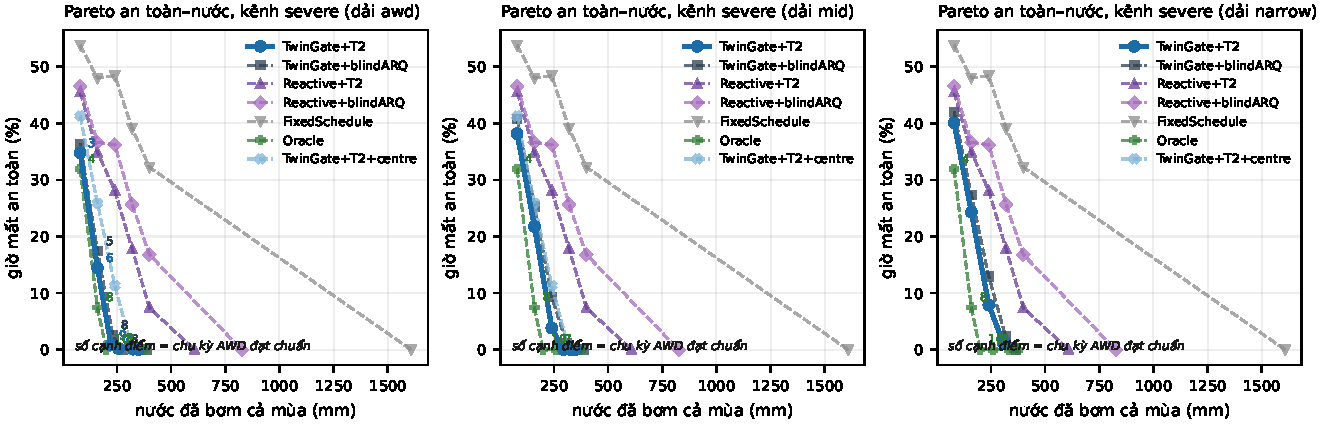
\includegraphics[width=0.72\textwidth]{fig8_pareto.pdf}
\caption{Mặt Pareto an toàn--nước cho cả bảy chính sách, kênh severe, ba dải độ trung thực. Mỗi điểm là một mức ngân sách; số cạnh điểm là số chu kỳ khô--ướt đạt chuẩn 72 giờ. Chính sách đề xuất (đường liền) nằm dưới-trái mọi mốc cơ sở trong vùng ngân sách ràng buộc.}
\label{fig:pareto}
\end{figure}

\subsection{Ý nghĩa thống kê (Wilcoxon ghép cặp, hiệu chỉnh Holm)}
\label{sec:wilcoxon}

Bảng~\ref{tab:wilcox} tổng hợp \textbf{540 so sánh ghép cặp} (108 ô $\times$ 5 mốc; trong mỗi ô các chính sách chạy cùng hạt giống): 344 khác biệt có ý nghĩa sau hiệu chỉnh Holm, 351 so sánh có trung vị âm, 121 so sánh hòa tuyệt đối, và \emph{không ô nào} cổng đề xuất thua có ý nghĩa. Với $n=10$ hạt giống, $p$ nhỏ nhất đạt được là $0{,}002$ nên chúng tôi báo cáo $p\le0{,}010$ thay vì ``$p<0{,}001$''.

\begin{table}[t]
\centering
\caption{Wilcoxon ghép cặp (Holm trong mỗi ô), cổng đề xuất so với từng mốc; ``ô có ý nghĩa'' đếm trên 6 ô mỗi dòng (3 trạm $\times$ 2 kênh); $\Delta$ âm nghĩa là cổng đề xuất ít giờ mất an toàn hơn.}
\label{tab:wilcox}
\scriptsize
% Sinh TU DONG tu outputs/*.csv boi experiments/make_latex_tables.py
% KHONG sua tay: moi con so deu truy nguon duoc ve CSV.

\begin{tabular}{@{}llcccc@{}}
\toprule
Dải $f_\sigma$ & Mốc so sánh với cổng đề xuất & Số ô & Ô có ý nghĩa & Trung vị $\Delta$ (điểm) & $|r|$ TB \\
\midrule
$0{,}02$ & centre-seeking (đối chứng luật chọn lệnh) & 36 & 18 & $-2{,}74$ & $0{,}89$ \\
$0{,}02$ & gửi lại mù (đối chứng T2) & 36 & 11 & 0 (hòa tuyệt đối) & $0{,}82$ \\
$0{,}02$ & ngưỡng tĩnh + T2 & 36 & 29 & $-14{,}16$ & $0{,}89$ \\
$0{,}02$ & ngưỡng tĩnh + gửi lại mù & 36 & 30 & $-18{,}46$ & $0{,}89$ \\
$0{,}02$ & lịch cố định (tập quán) & 36 & 30 & $-31{,}08$ & $0{,}89$ \\
\addlinespace[2pt]
$0{,}05$ & centre-seeking (đối chứng luật chọn lệnh) & 36 & 18 & $-0{,}72$ & $0{,}88$ \\
$0{,}05$ & gửi lại mù (đối chứng T2) & 36 & 18 & $-0{,}29$ & $0{,}87$ \\
$0{,}05$ & ngưỡng tĩnh + T2 & 36 & 29 & $-12{,}03$ & $0{,}89$ \\
$0{,}05$ & ngưỡng tĩnh + gửi lại mù & 36 & 30 & $-14{,}00$ & $0{,}89$ \\
$0{,}05$ & lịch cố định (tập quán) & 36 & 30 & $-29{,}20$ & $0{,}89$ \\
\addlinespace[2pt]
$0{,}10$ & centre-seeking (đối chứng luật chọn lệnh) & 36 & 0 & 0 (hòa tuyệt đối) & -- \\
$0{,}10$ & gửi lại mù (đối chứng T2) & 36 & 12 & 0 (hòa tuyệt đối) & $0{,}80$ \\
$0{,}10$ & ngưỡng tĩnh + T2 & 36 & 29 & $-9{,}88$ & $0{,}88$ \\
$0{,}10$ & ngưỡng tĩnh + gửi lại mù & 36 & 30 & $-12{,}95$ & $0{,}89$ \\
$0{,}10$ & lịch cố định (tập quán) & 36 & 30 & $-27{,}82$ & $0{,}89$ \\
\addlinespace[2pt]
\bottomrule
\end{tabular}

\end{table}

Hai điểm cần đọc kỹ. \emph{Luật chọn lệnh thích ứng} có ý nghĩa ở 18/36 ô dải $f_\sigma{=}0{,}02$ và 18/36 ô dải $0{,}05$, nhưng \textbf{0/36 ô} dải $0{,}10$ (hòa tuyệt đối cả 36), qua đó xác nhận thực nghiệm Mệnh đề~\ref{prop:dmax}: khi vùng đạt hẹp hơn bước nhảy ứng viên (4,2 so với 20\,mm) thì mọi luật chọn lệnh trả về cùng một lệnh. Lợi ích của luật này \emph{có điều kiện} về độ trung thực, và điều kiện đó tính được bằng công thức. \emph{T2 so với gửi lại mù} thắng cả hai chỉ số tại các ô ràng buộc ($f_\sigma{=}0{,}02$, severe, $B{=}240$: nước lãng phí do tưới đúp 72,0 $\to$ 55,3\,mm; giờ mất an toàn 2,48 $\to$ 0,81\%); ở các ô không ràng buộc hai cơ chế hòa nhau vì nước không còn khan, nên lợi ích còn lại của T2 là tài nguyên vô tuyến (Bảng~\ref{tab:deploy}).

\subsection{Mặt ngưỡng $f_\sigma \times \delta$ (kiểm chứng Hệ quả~\ref{cor:sigma} và Mệnh đề~\ref{prop:dmax})}
\label{sec:sweep}

Quét $f_\sigma$ trên tám mức 0,02--0,20 kết hợp $\delta$ trên sáu mức 0,01--0,20 với cả hai luật chọn lệnh: \textbf{11\,520 lần mô phỏng} tại hai mức ngân sách (Bảng~\ref{tab:sweep80}).

\begin{table}[t]
\centering
\caption{Giờ mất an toàn (\%) trên mặt $(f_\sigma,\delta)$; severe, $B{=}80$\,mm, chính sách đề xuất. Mức 57,8\% $=$ ``cổng rỗng'', bằng mức ruộng không được tưới.}
\label{tab:sweep80}
\scriptsize
% Sinh TU DONG tu outputs/*.csv boi experiments/make_latex_tables.py
% KHONG sua tay: moi con so deu truy nguon duoc ve CSV.

\begin{tabular}{@{}lcccccc@{}}
\toprule
$\sigma_{frac}$ \textbackslash\ $\delta$ & 0.01 & 0.03 & 0.05 & 0.1 & 0.15 & 0.2 \\
\midrule
0.02 & $36{,}5$ & $35{,}9$ & $34{,}8$ & $32{,}8$ & $32{,}7$ & $31{,}7$ \\
0.03 & $37{,}9$ & $37{,}4$ & $36{,}9$ & $35{,}9$ & $34{,}5$ & $32{,}8$ \\
0.05 & $40{,}2$ & $38{,}8$ & $38{,}2$ & $37{,}5$ & $36{,}8$ & $36{,}1$ \\
0.08 & $40{,}2$ & $41{,}0$ & $40{,}9$ & $39{,}2$ & $38{,}1$ & $37{,}7$ \\
0.1 & $57{,}8$ & $57{,}8$ & $40{,}1$ & $40{,}9$ & $39{,}4$ & $38{,}4$ \\
0.12 & $57{,}8$ & $57{,}8$ & $57{,}8$ & $40{,}2$ & $40{,}8$ & $39{,}2$ \\
0.15 & $57{,}8$ & $57{,}8$ & $57{,}8$ & $57{,}8$ & $57{,}8$ & $41{,}1$ \\
0.2 & $57{,}8$ & $57{,}8$ & $57{,}8$ & $57{,}8$ & $57{,}8$ & $57{,}8$ \\
\bottomrule
\end{tabular}

\end{table}

Giờ mất an toàn rơi vào đúng \textbf{hai chế độ}, hoặc ``chết'' ở 57,8\% (cổng rỗng, không phát lệnh nào) hoặc ``sống'' ở 31,7--41,1\%. Ranh giới bám $\sigma_H \approx \sigma^{*}$ như Hệ quả~\ref{cor:sigma} dự đoán: $(f_\sigma{=}0{,}10;\delta\le0{,}03)$ chết nhưng $(\delta\ge0{,}05)$ sống vì $z_{1-\delta/2}$ giảm kéo $\sigma^{*}$ lên; $f_\sigma{=}0{,}20$ chết ở mọi $\delta$ trong vùng quét.

Mệnh đề~\ref{prop:dmax} được kiểm chứng ở cấp episode: tại các ô vùng đạt hẹp hơn bước nhảy ứng viên, hai luật chọn lệnh cho kết quả \emph{giống hệt nhau} ở 94/104 ô (90,4\%); tại các ô vùng đạt rộng, chúng khác nhau ở 53/88 ô (60,2\%). Mười ô ngoại lệ đều ở ngân sách khan nhất với \emph{cùng tổng nước, cùng số lệnh}; khác biệt chỉ ở thời điểm phát lệnh, nhất quán với việc bucket bị chặn ở dung trọng đồng ruộng làm $\mu(u)$ của hai ứng viên trùng nhau (đo trực tiếp: 4/7 mức depletion có ít nhất hai ứng viên cùng $\mu$).

Hai giới hạn ghi nhận trung thực: (i) mặt ngưỡng có dạng \emph{bước nhảy} chứ không trơn do tập ứng viên rời rạc; (ii) $\delta$ nới lỏng làm giờ mất an toàn toàn mùa \emph{giảm} ở 46 ô có ý nghĩa thống kê (0,18--19,6 điểm), vì ở chế độ khan nguyên nhân chính của ``mất an toàn'' là không được tưới. Đó là đánh đổi vận hành thật, khi bảo đảm trên từng lệnh yếu đi còn tổng nước tới ruộng tăng, chứ không mâu thuẫn Định lý~\ref{thm:t1} (vốn phát biểu trên từng lệnh được phát).

\subsection{AWD đạt chuẩn và ``giá của chứng chỉ''}
\label{sec:awd}

Ràng buộc vận hành của QĐ 4801, theo đó rút nước chỉ được coi là hiệu quả nếu ruộng không bị tưới lại trong ít nhất ba ngày, được mã hóa thành chỉ số đo chính: mỗi chu kỳ chỉ được đếm là \emph{đạt chuẩn} khi pha khô kéo dài $\ge$72 giờ. Bảng~\ref{tab:awd} cho kết quả theo dải độ trung thực và ngân sách.

\begin{table}[t]
\centering
\caption{Chu kỳ AWD đạt chuẩn $\ge$72 giờ (QĐ 4801); chính sách đề xuất, severe, 30 lần mô phỏng mỗi ô. ``Hụt chuẩn'' $=$ pha khô $<$72 giờ nên không được tính tín chỉ.}
\label{tab:awd}
\scriptsize
% Sinh TU DONG tu outputs/*.csv boi experiments/make_latex_tables.py
% KHONG sua tay: moi con so deu truy nguon duoc ve CSV.

\begin{tabular}{@{}llcccc@{}}
\toprule
Dải $f_\sigma$ & Ngân sách $B$ (mm) & AWD đạt chuẩn & AWD hụt chuẩn & giờ stress & mất an toàn (\%) \\
\midrule
$0{,}02$ & 80 & $3{,}17$ & $0{,}00$ & $1596$ & $34{,}79$ \\
 & 240 & $8{,}73$ & $0{,}00$ & $1402$ & $0{,}81$ \\
 & 400 & $1{,}97$ & $7{,}77$ & $731$ & $0{,}10$ \\
 & $\infty$ & $0{,}17$ & $9{,}03$ & $544$ & $0{,}02$ \\
\addlinespace[2pt]
$0{,}05$ & 80 & $0{,}57$ & $2{,}83$ & $1544$ & $38{,}17$ \\
 & 240 & $1{,}23$ & $8{,}83$ & $1308$ & $3{,}84$ \\
 & 400 & $0{,}70$ & $9{,}80$ & $751$ & $0{,}02$ \\
 & $\infty$ & $0{,}17$ & $9{,}03$ & $544$ & $0{,}02$ \\
\addlinespace[2pt]
$0{,}10$ & 80 & $0{,}27$ & $2{,}93$ & $1502$ & $40{,}07$ \\
 & 240 & $0{,}53$ & $9{,}33$ & $1183$ & $7{,}91$ \\
 & 400 & $0{,}53$ & $11{,}87$ & $858$ & $1{,}32$ \\
 & $\infty$ & $0{,}53$ & $11{,}87$ & $858$ & $1{,}32$ \\
\addlinespace[2pt]
\bottomrule
\end{tabular}

\end{table}

Hai kết quả cần đọc cùng nhau. \emph{Thứ nhất}, độ trung thực quyết định tính khả thi: tại dải $f_\sigma{=}0{,}02$ với $B{=}240$\,mm, cổng tạo \textbf{8,73 chu kỳ đạt chuẩn} mỗi mùa và 0 chu kỳ hụt; tại dải $f_\sigma{=}0{,}10$ chỉ còn 0,27--0,53 chu kỳ bất kể ngân sách. Ngưỡng $f_\sigma \le 0{,}025$ suy ra từ công thức (Bảng~\ref{tab:spec}) khớp với điểm gãy này. \emph{Thứ hai}, và ngược trực giác: \emph{tăng} ngân sách làm \emph{giảm} số chu kỳ đạt chuẩn (8,73 $\to$ 1,97 $\to$ 0,17 khi $B$ tăng 240 $\to$ 400 $\to \infty$) trong khi giờ stress cây cũng giảm (1\,177 $\to$ 566). Cơ chế: khi nước không khan, luật thích ứng tự chuyển sang tối đa biên an toàn nên tưới sớm, pha khô bị cắt dưới 72 giờ và mất tư cách tín chỉ. Đây là \textbf{giá của chứng chỉ các-bon}; cùng một cơ chế không thể đồng thời tối đa an toàn/năng suất và tối đa số chu kỳ AWD đủ điều kiện, và người vận hành phải chọn theo mục tiêu. Chúng tôi coi việc lượng hóa được sự đánh đổi này, chứ không phải việc đạt cả hai, là đóng góp của bài.

\subsection{Kiểm chứng bằng bất biến}
\label{sec:invariants}

Bất biến I6 (tắt hoàn toàn việc tái neo): $\sigma$ vượt $\sigma^{*}{=}15{,}18$\,mm, dẫn tới 0 lệnh, tỷ lệ mất an toàn 57,82\% và sai số căn quân phương RMSE (root-mean-square error) giữa bản sao số và ruộng thật bằng 0,000. Tuy nhiên đây là \emph{sự trùng khớp suy biến} (degenerate agreement) do cả hai đều không nhận nước chứ không phải độ chính xác; một kiểm định dạng ``RMSE giảm khi bật bản sao số'' sẽ thưởng cho con số không này và đã được chúng tôi viết lại thành bất biến đúng. Bất biến I7 (hiệu chuẩn): tỷ lệ bao phủ thực nghiệm của dải chuẩn hóa 95\% là 0,9906--1,0000 (với $n{=}6480$ mẫu mỗi ô), suy ra $\sigma$ hơi bảo thủ. Theo nguyên tắc bảo thủ (conservativeness) tại Mục 9.3 của VM0051~\cite{vm0051} thì đây là sai lệch về phía an toàn, nhưng vẫn là một hạn chế vì cổng im lặng nhiều hơn mức tối ưu. Các bất biến I1--I5 đều đạt.

\subsection{Kết luận có điều kiện từ hai năm khí hậu}
\label{sec:twoyears}

Mùa khô 2025 ướt hơn 2024 rõ rệt: thiếu hụt ròng vật lý ($K_c\sum ET_0 - \sum P$) chỉ còn 0--158\,mm so với 302--318\,mm của 2024. Trên lưới đầy đủ 7\,560 lần mô phỏng của năm 2025, tại ngân sách khan nhất $B{=}80$ (kênh severe), giờ mất an toàn của TwinGate+T2 ở dải $f_\sigma{=}0{,}02$ là \textbf{2,29\%} so với Reactive+T2 9,89\% và FixedSchedule 20,20\%; mốc Oracle là 2,20\%, tức khoảng cách tới thông tin hoàn hảo gần như biến mất vì nước không còn khan. Kiểm định Wilcoxon trên 540 so sánh của năm 2025: 174 khác biệt có ý nghĩa, 270 ô hòa tuyệt đối (mọi chính sách cùng đạt 0 vi phạm khi nước dư), và \emph{không ô nào} chính sách đề xuất thua có ý nghĩa thống kê.

Kết luận vì vậy phải được phát biểu có điều kiện: \textbf{cổng không bao giờ thua; thắng đậm khi nước khan (2024) và hòa khi nước dư (2025)}. Việc gộp hai năm thành một con số duy nhất sẽ thổi phồng hiệu quả.

\subsection{Ràng buộc C2 về mặn theo triều và giá của việc chờ con nước}
\label{sec:salinity}

Cửa sổ sốc nhiệt III--V trùng đỉnh xâm nhập mặn ở ĐBSCL~\cite{mard2025sal}, và nguồn ngọt chỉ hiện diện trong một phần chu kỳ triều bán nhật ($M_2$, 12,4206\,giờ). Vì \emph{không có} số đo mặn thực địa tại ba trạm, chúng tôi không khẳng định giá trị mặn cụ thể nào: toàn bộ mục này là \textbf{phân tích tình huống}, với cường độ xâm nhập $i \in \{0{,}25;\ldots;2{,}0\}$ và ba biến thể ngưỡng chịu mặn EC$_{crit}$ quét đầy đủ (Grattan 1,9; trung tâm 2,5; Maas 3,5\,dS/m cho giai đoạn trổ, giai đoạn mà văn liệu còn tranh cãi)~\cite{maas1977,usdaP572}. Cách làm này dịch chuyển phát biểu khoa học từ ``độ mặn là $x$'' sang ``kết luận đúng trong khoảng tham số nào'', và là lý do mục này không vào phần tóm tắt như một kết quả chính.

\begin{table}[t]
\centering
\caption{Tình huống xâm nhập mặn (1\,800 lần mô phỏng); severe, ngưỡng trung tâm, ba trạm. \textbf{Không có số đo thực địa}, giá trị là của mô hình tình huống.}
\label{tab:sal}
\scriptsize
\resizebox{\textwidth}{!}{% Sinh TU DONG tu outputs/*.csv boi experiments/make_latex_tables.py
% KHONG sua tay: moi con so deu truy nguon duoc ve CSV.

\begin{tabular}{@{}llcccccc@{}}
\toprule
Cường độ $i$ & Chính sách & nước mặn (mm) & muối thừa (dS$\cdot$mm) & thiệt hại NS (\%) & mất an toàn (\%) & im lặng (chu kỳ) & giờ ngọt (\%) \\
\midrule
0{,}25 & \textbf{Cổng đề xuất} & $0{,}0$ & $0$ & $0{,}0$ & $7{,}81$ & $0{,}0$ & $87{,}8$ \\
 & ngưỡng tĩnh + T2 & $24{,}0$ & $4$ & $0{,}9$ & $27{,}28$ & $0{,}0$ & $87{,}8$ \\
 & lịch cố định & $0{,}0$ & $0$ & $0{,}0$ & $47{,}72$ & $0{,}0$ & $87{,}8$ \\
 & Oracle & $0{,}0$ & $0$ & $0{,}0$ & $0{,}03$ & $0{,}0$ & $87{,}8$ \\
\addlinespace[2pt]
0{,}50 & \textbf{Cổng đề xuất} & $0{,}0$ & $0$ & $0{,}0$ & $8{,}35$ & $0{,}0$ & $49{,}7$ \\
 & ngưỡng tĩnh + T2 & $128{,}0$ & $196$ & $19{,}0$ & $27{,}28$ & $0{,}0$ & $49{,}7$ \\
 & lịch cố định & $132{,}0$ & $150$ & $14{,}0$ & $47{,}72$ & $0{,}0$ & $49{,}7$ \\
 & Oracle & $0{,}0$ & $0$ & $0{,}0$ & $0{,}00$ & $0{,}0$ & $49{,}7$ \\
\addlinespace[2pt]
1{,}00 & \textbf{Cổng đề xuất} & $0{,}0$ & $0$ & $0{,}0$ & $27{,}29$ & $29{,}0$ & $19{,}4$ \\
 & ngưỡng tĩnh + T2 & $180{,}0$ & $780$ & $53{,}8$ & $27{,}28$ & $0{,}0$ & $19{,}4$ \\
 & lịch cố định & $192{,}0$ & $731$ & $45{,}2$ & $47{,}72$ & $0{,}0$ & $19{,}4$ \\
 & Oracle & $0{,}0$ & $0$ & $0{,}0$ & $27{,}86$ & $29{,}0$ & $19{,}4$ \\
\addlinespace[2pt]
1{,}50 & \textbf{Cổng đề xuất} & $0{,}0$ & $0$ & $0{,}0$ & $28{,}91$ & $32{,}1$ & $9{,}1$ \\
 & ngưỡng tĩnh + T2 & $220{,}0$ & $1430$ & $79{,}3$ & $27{,}28$ & $0{,}0$ & $9{,}1$ \\
 & lịch cố định & $240{,}0$ & $1410$ & $70{,}5$ & $47{,}72$ & $0{,}0$ & $9{,}1$ \\
 & Oracle & $0{,}0$ & $0$ & $0{,}0$ & $31{,}65$ & $33{,}7$ & $9{,}1$ \\
\addlinespace[2pt]
2{,}00 & \textbf{Cổng đề xuất} & $0{,}0$ & $0$ & $0{,}0$ & $54{,}12$ & $61{,}0$ & $2{,}6$ \\
 & ngưỡng tĩnh + T2 & $240{,}0$ & $2116$ & $96{,}4$ & $27{,}28$ & $0{,}0$ & $2{,}6$ \\
 & lịch cố định & $240{,}0$ & $2096$ & $89{,}7$ & $47{,}72$ & $0{,}0$ & $2{,}6$ \\
 & Oracle & $0{,}0$ & $0$ & $0{,}0$ & $54{,}12$ & $61{,}3$ & $2{,}6$ \\
\addlinespace[2pt]
\bottomrule
\end{tabular}
}
\end{table}

\begin{figure}[t]
\centering
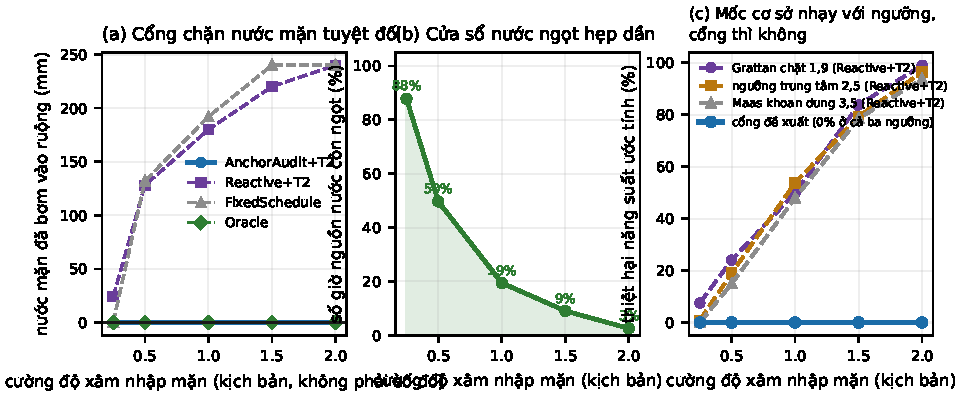
\includegraphics[width=0.70\textwidth]{fig7_salinity_scenario.pdf}
\caption{Phân tích tình huống xâm nhập mặn (1\,800 lần mô phỏng, \textbf{không phải số đo thực địa}). (a) Nước mặn bơm vào ruộng: cổng loại trừ tuyệt đối ở mọi mức xâm nhập, các mốc không nhìn chất lượng nguồn tích lũy tới 240\,mm. (b) Cửa sổ nước ngọt hẹp dần theo cường độ xâm nhập. (c) Thiệt hại năng suất của mốc cơ sở theo ba bảng ngưỡng chịu mặn khác nhau, trong khi cổng đề xuất cho 0\% ở cả ba.}
\label{fig:salinity}
\end{figure}

Bảng~\ref{tab:sal} và Hình~\ref{fig:salinity} cho thấy cổng \emph{không bao giờ} bơm nước mặn (0,00\,mm và 0,00\% thiệt hại năng suất ở mọi mức xâm nhập), trong khi Reactive+T2 bơm 24--240\,mm (thiệt hại 0,9--96,4\%) và FixedSchedule 132--240\,mm (14,0--89,7\%). Giá của việc chờ con nước, đo bằng chênh lệch giờ mất an toàn so với Reactive+T2, \emph{đổi dấu} theo cường độ: cổng thắng ở mức nhẹ ($i{=}0{,}25$: $-19{,}5$ điểm; $i{=}0{,}5$: $-18{,}9$), hòa ở mức điển hình ($i{=}1{,}0$: $+0{,}01$ điểm, trong khi tránh 780\,dS$\cdot$mm muối và 53,8 điểm thiệt hại năng suất), rồi trả giá thật ở mức gắt ($i{=}1{,}5$: $+1{,}6$; $i{=}2{,}0$: $+26{,}8$ điểm để tránh 2\,116\,dS$\cdot$mm khi cửa sổ ngọt chỉ còn 2,6\% số giờ và cổng im lặng 61 chu kỳ). Ở $i{=}2$, giờ mất an toàn của cổng (54,12\%) bằng đúng mức ruộng không được tưới, là hiện thân thứ hai của Hệ quả~\ref{cor:sigma}, lần này nguyên nhân nằm ở \emph{nguồn nước} thay vì bản sao số.

\begin{table}[t]
\centering
\caption{Thiệt hại năng suất (\%) theo ba bảng ngưỡng chịu mặn; severe. Cổng đề xuất 0\% ở cả ba nên \emph{miễn nhiễm} với tranh cãi về ngưỡng; mốc cơ sở nhạy rõ.}
\label{tab:salthresh}
\scriptsize
% Sinh TU DONG tu outputs/*.csv boi experiments/make_latex_tables.py
% KHONG sua tay: moi con so deu truy nguon duoc ve CSV.

\begin{tabular}{@{}llccccc@{}}
\toprule
Chính sách & Bảng ngưỡng EC$_{crit}$ (dS/m) & $i=0{,}25$ & $i=0{,}50$ & $i=1{,}00$ & $i=1{,}50$ & $i=2{,}00$ \\
\midrule
\textbf{Cổng đề xuất} & trung tâm 2,5 & $0{,}0$ & $0{,}0$ & $0{,}0$ & $0{,}0$ & $0{,}0$ \\
 & Grattan chặt 1,9 & $0{,}0$ & $0{,}0$ & $0{,}0$ & $0{,}0$ & $0{,}0$ \\
 & Maas khoan dung 3,5 & $0{,}0$ & $0{,}0$ & $0{,}0$ & $0{,}0$ & $0{,}0$ \\
\addlinespace[2pt]
ngưỡng tĩnh + T2 & trung tâm 2,5 & $0{,}9$ & $19{,}0$ & $53{,}8$ & $79{,}3$ & $96{,}4$ \\
 & Grattan chặt 1,9 & $7{,}5$ & $24{,}0$ & $50{,}0$ & $83{,}7$ & $99{,}0$ \\
 & Maas khoan dung 3,5 & $0{,}0$ & $14{,}9$ & $47{,}9$ & $78{,}4$ & $93{,}8$ \\
\addlinespace[2pt]
\bottomrule
\end{tabular}

\end{table}

Bảng~\ref{tab:salthresh} nêu một tính chất đáng giá: với cổng đề xuất, cả ba bảng EC$_{crit}$ cho kết quả \emph{giống hệt nhau}, vì cổng loại trừ tuyệt đối mọi lệnh trong giờ mặn nên ngưỡng không bao giờ được dùng tới. Ngược lại các mốc cơ sở nhạy rõ với ngưỡng, nên việc chọn ngưỡng vẫn là vấn đề đối với cách làm truyền thống. Toàn bộ mục này là phân tích tình huống, không phải kết luận về mức tuân thủ thực tế.

\subsection{Ablation và cái giá của từng thành phần}
\label{sec:ablation}

Mỗi thành phần phải tự chứng minh đóng góp: chúng tôi tắt lần lượt từng thành phần trên cùng hạt giống, cùng thời tiết, cùng chuỗi sự kiện kênh (4\,800 lần mô phỏng; Bảng~\ref{tab:abl}, Hình~\ref{fig:ablation}; tính trên ngân sách ràng buộc, kênh severe).

\begin{table}[t]
\centering
\caption{Ablation tại hai dải độ trung thực; mỗi dòng tắt \emph{đúng một} thành phần. ``Vùng đạt'' $=W-2z\sigma_H$: 48\,mm ở $f_\sigma{=}0{,}02$ so với 4\,mm ở $f_\sigma{=}0{,}10$ (hẹp hơn bước nhảy 20\,mm).}
\label{tab:abl}
\scriptsize
% Sinh TU DONG tu outputs/*.csv boi experiments/make_latex_tables.py
% KHONG sua tay: moi con so deu truy nguon duoc ve CSV.

\begin{tabular}{@{}lcccccc@{}}
\toprule
 & \multicolumn{3}{c}{$f_\sigma=0{,}02$ (vùng đạt rộng 48\,mm)} & \multicolumn{3}{c}{$f_\sigma=0{,}10$ (vùng đạt hẹp 4\,mm)} \\
\cmidrule(lr){2-4}\cmidrule(lr){5-7}
Biến thể (tắt đúng một thành phần) & mất an toàn (\%) & nước đúp (mm) & AWD đạt & mất an toàn (\%) & nước đúp (mm) & AWD đạt \\
\midrule
\textbf{Đầy đủ (cơ chế đề xuất)} & $12{,}58$ & $45{,}8$ & $6{,}42$ & $18{,}39$ & $44{,}0$ & $0{,}42$ \\
bỏ tính phản thực (twin $\to$ predictor) & $52{,}75$ & $44{,}7$ & $0{,}00$ & $45{,}19$ & $31{,}0$ & $0{,}40$ \\
bỏ cổng ràng buộc cơ hội & $31{,}57$ & $24{,}3$ & $0{,}10$ & $31{,}57$ & $24{,}3$ & $0{,}10$ \\
bỏ luật chọn lệnh thích ứng & $19{,}62$ & $48{,}5$ & $0{,}17$ & $18{,}39$ & $44{,}0$ & $0{,}42$ \\
bỏ tái neo bằng cảm biến & $16{,}87$ & $46{,}5$ & $4{,}12$ & $57{,}81$ & $0{,}0$ & $0{,}00$ \\
bỏ T2 (gửi lại mù) & $14{,}07$ & $61{,}7$ & $5{,}92$ & $21{,}15$ & $65{,}5$ & $0{,}00$ \\
bỏ trần chu kỳ 24 giờ & $13{,}99$ & $52{,}0$ & $5{,}74$ & $20{,}43$ & $49{,}2$ & $0{,}00$ \\
Oracle (thông tin hoàn hảo) & $9{,}85$ & $24{,}0$ & $7{,}32$ & $9{,}85$ & $24{,}0$ & $7{,}32$ \\
\bottomrule
\end{tabular}

\end{table}

Thứ tự đóng góp theo giờ mất an toàn ở dải $f_\sigma{=}0{,}02$: bỏ tính phản thực của bản sao số (rollout với $u{=}0$, tức ``twin'' thoái hóa thành predictor) tăng \textbf{$+36{,}90$} điểm; bỏ cổng ràng buộc cơ hội $+19{,}47$; bỏ luật chọn lệnh thích ứng $+9{,}46$; bỏ tái neo cảm biến $+4{,}13$; bỏ T2 $+2{,}07$ kèm nước lãng phí do tưới đúp tăng 38,7 $\to$ 50,0\,mm; bỏ trần chu kỳ 24 giờ $+1{,}96$. Mọi thành phần đều có đóng góp đo được ở ít nhất một dải; riêng luật thích ứng vô hiệu ở dải $f_\sigma{=}0{,}10$ đúng như Mệnh đề~\ref{prop:dmax} dự đoán, và điều đó được báo cáo như một phần kết quả chứ không bị giấu. Đóng góp của T2 thể hiện rõ nhất trên \emph{nước lãng phí do tưới đúp} chứ không phải giờ mất an toàn, đúng bản chất cơ chế niềm tin $\pi$ (chặn tưới trùng khi không chắc lệnh cũ đã tới).

\begin{figure}[t]
\centering
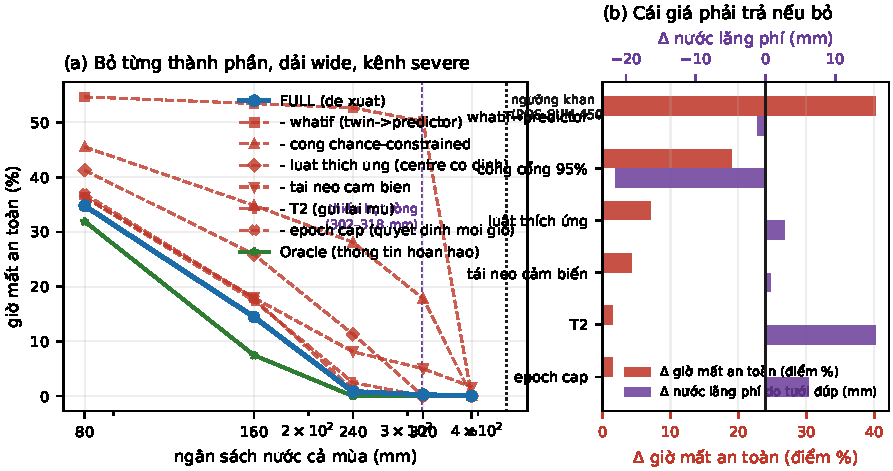
\includegraphics[width=0.70\textwidth]{fig2_ablation.pdf}
\caption{Ablation tại dải $f_\sigma=0{,}02$, kênh severe, ngân sách ràng buộc: (a) giờ mất an toàn theo ngân sách khi tắt từng thành phần; (b) cái giá của mỗi thành phần trên hai chỉ số.}
\label{fig:ablation}
\end{figure}

\subsection{Điều kiện để hệ thống chạy được ngoài đồng}
\label{sec:deploy}

Năm yếu tố triển khai được quét riêng từng yếu tố (540 lần mô phỏng; Bảng~\ref{tab:deploy}, Hình~\ref{fig:deploy}), kèm \textbf{ô đặc tả} suy ra bằng công thức (Bảng~\ref{tab:spec}).

\begin{table}[t]
\centering
\caption{Quét một yếu tố tại một thời điểm ($f_\sigma{=}0{,}02$; $B{=}240$\,mm; 3 trạm $\times$ 2 kênh $\times$ 5 hạt giống).}
\label{tab:deploy}
\scriptsize
\resizebox{\textwidth}{!}{% Sinh TU DONG tu outputs/*.csv boi experiments/make_latex_tables.py
% KHONG sua tay: moi con so deu truy nguon duoc ve CSV.

\begin{tabular}{@{}llccccc@{}}
\toprule
Yếu tố & Mức & mất an toàn (\%) & AWD đạt & giờ stress & lệnh/ngày & gửi lại/ngày \\
\midrule
Mất gói uplink & 5\% & $0{,}28$ & $9{,}10$ & $1387$ & $0{,}120$ & $0{,}128$ \\
 & 15\% & $0{,}28$ & $9{,}07$ & $1381$ & $0{,}120$ & $0{,}127$ \\
 & 30\% & $0{,}28$ & $9{,}00$ & $1373$ & $0{,}121$ & $0{,}128$ \\
 & 50\% & $0{,}33$ & $8{,}97$ & $1361$ & $0{,}120$ & $0{,}129$ \\
 & 70\% & $0{,}45$ & $8{,}93$ & $1358$ & $0{,}120$ & $0{,}131$ \\
 & 90\% & $0{,}54$ & $8{,}80$ & $1383$ & $0{,}122$ & $0{,}140$ \\
\addlinespace[2pt]
Loại đất & cát pha & $0{,}00$ & $7{,}50$ & $1423$ & $0{,}111$ & $0{,}128$ \\
 & thịt pha sét & $0{,}28$ & $9{,}07$ & $1381$ & $0{,}120$ & $0{,}127$ \\
 & sét & $0{,}07$ & $8{,}80$ & $1419$ & $0{,}122$ & $0{,}148$ \\
\addlinespace[2pt]
Độ phân giải lệnh & nông học $\{20,40,60\}$ & $0{,}28$ & $9{,}07$ & $1381$ & $0{,}120$ & $0{,}127$ \\
 & mịn $\{10,20,35\}$ & $0{,}23$ & $4{,}43$ & $1469$ & $0{,}194$ & $0{,}214$ \\
 & thô $\{35,60,90\}$ & $9{,}65$ & $5{,}07$ & $1274$ & $0{,}069$ & $0{,}078$ \\
\addlinespace[2pt]
Chân trời dự báo $H$ & 3 ngày & $0{,}32$ & $9{,}03$ & $1402$ & $0{,}119$ & $0{,}134$ \\
 & 6 ngày & $0{,}28$ & $9{,}07$ & $1381$ & $0{,}120$ & $0{,}127$ \\
 & 12 ngày & $0{,}45$ & $8{,}53$ & $1342$ & $0{,}126$ & $0{,}136$ \\
 & 24 ngày & $0{,}97$ & $4{,}43$ & $1361$ & $0{,}138$ & $0{,}160$ \\
\addlinespace[2pt]
Kiểu gửi lại & T2 (đề xuất) & $0{,}28$ & $9{,}07$ & $1381$ & $0{,}120$ & $0{,}127$ \\
 & gửi lại mù & $3{,}19$ & $8{,}03$ & $1363$ & $0{,}089$ & $0{,}199$ \\
\addlinespace[2pt]
\bottomrule
\end{tabular}
}
\end{table}

Về chất lượng mạng, giờ mất an toàn chỉ tăng 0,28 $\to$ 0,54\% khi mất gói uplink tăng 5 $\to$ 90\%, nghĩa là cổng chịu được mạng cảm biến rất kém vì im lặng vốn là hành vi an toàn mặc định. Về loại đất, kết quả ổn định (0,00--0,28\%) nhưng ngưỡng AWD đổi theo đất ($W$ từ 59,5 lên 80,8\,mm với đất cát pha kéo $\sigma^{*}$ từ 15,18 lên 20,60\,mm), tức đất cát \emph{dễ} đạt chuẩn AWD hơn với cùng một bản sao số. \emph{Độ phân giải lệnh} là yếu tố ăn tiền nhất: van chỉ mở mức thô $\{35;60;90\}$\,mm làm mất an toàn tăng 0,28 $\to$ \textbf{9,65\%}, trong khi mức mịn $\{10;20;35\}$ không tốt hơn mức nông học $\{20;40;60\}$ (0,23 so với 0,28\%) mà đòi gấp 1,6 lần số lệnh, nên thiết bị mức 20\,mm là đủ và kinh tế nhất. Về chân trời dự báo, $H{=}6$ giờ là tối ưu; $H{=}24$ làm mất an toàn tăng lên 0,97\% và chu kỳ AWD đạt chuẩn giảm 9,0 $\to$ 4,4 vì dự báo xa làm $\sigma_H$ phình. Về tài nguyên vô tuyến, T2 gửi lại 0,127 lần/ngày so với 0,199 của gửi lại mù ($-36\%$) mà giờ mất an toàn vẫn thấp hơn (0,28 so với 3,19\%).

\begin{table}[t]
\centering
\caption{Ô đặc tả, trong đó mọi ngưỡng suy ra bằng công thức từ $W$, TAW, $\rho$, $z$ chứ không thử--sai. Đất tham chiếu là thịt pha sét với TAW $=70$\,mm.}
\label{tab:spec}
\scriptsize
% Sinh TU DONG tu outputs/*.csv boi experiments/make_latex_tables.py
% KHONG sua tay: moi con so deu truy nguon duoc ve CSV.

\begin{tabular}{@{}lll@{}}
\toprule
Đại lượng & Công thức & Giá trị \\
\midrule
$W$ (chiều rộng tập an toàn) & $(0{,}85-0)\times$TAW & $59{,}5$\,mm \\
$\sigma^{*}$ (ngưỡng cổng rỗng) & $W/(2z_{1-\delta/2})$ & $15{,}18$\,mm \\
$\sigma_H$ tối thiểu (tuổi 0) & $f_\sigma\cdot$TAW$\cdot\sqrt{\sum\rho^{2k}}$ & $f_\sigma\times141{,}03$\,mm \\
$\sigma$ tĩnh (tuổi $\infty$) & $f_\sigma\cdot$TAW$/\sqrt{1-\rho^2}$ & $f_\sigma\times160{,}59$\,mm \\
$\sigma_H$ cần cho AWD ($d^*=0{,}75$) & $(0{,}85-d^{*})\cdot$$\mathrm{span}/z$ & $3{,}57$\,mm \\
$f_\sigma$ tối đa để cổng sống & $\sigma^{*}/(\mathrm{TAW}/\sqrt{1-\rho^2})$ & $0{,}0945$ \\
$f_\sigma$ tối đa để AWD đạt chuẩn (tuổi 0) & $\sigma_{\text{cần}}/(\mathrm{TAW}\cdot g)$ & $0{,}0253$ \\
$f_\sigma$ tối đa để AWD đạt chuẩn (tuổi $\infty$) & $\sigma_{\text{cần}}/\sigma_{\text{tĩnh}}$ & $0{,}0222$ \\
\bottomrule
\end{tabular}

\end{table}

Hai hệ quả triển khai từ Bảng~\ref{tab:spec}: (i) với bản sao số thô ($f_\sigma{=}0{,}10$), $\sigma_H$ có \emph{giới hạn dưới} 14,10\,mm ngay cả khi tuổi dữ liệu bằng 0, nên \textbf{tăng tần suất cảm biến không cứu được} mà phải cải thiện chính mô hình; (ii) với $f_\sigma{=}0{,}02$, $\sigma$ tĩnh chỉ 3,21\,mm nên cổng vẫn làm được AWD \emph{ngay cả khi không bao giờ được tái neo} (pin yếu, kênh nghẽn), nên cấu hình cảm biến tối thiểu vẫn khả thi về MRV.

\begin{figure}[t]
\centering
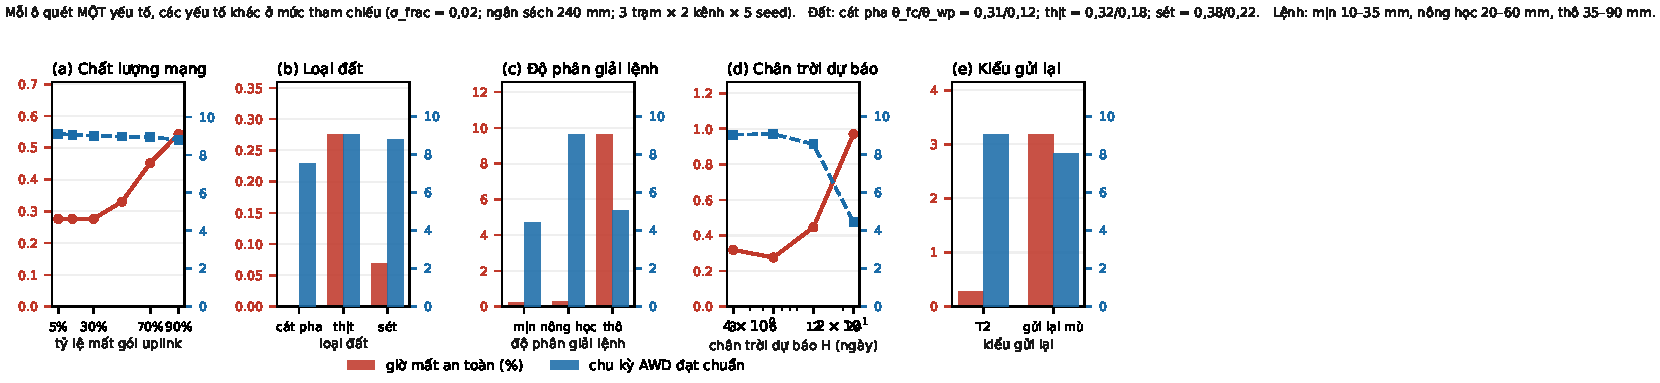
\includegraphics[width=0.72\textwidth]{fig5_deployment.pdf}
\caption{Năm yếu tố triển khai, mỗi ô quét một yếu tố, lần lượt là (a) mất gói uplink; (b) loại đất; (c) độ phân giải lệnh; (d) chân trời dự báo $H$; (e) T2 so với gửi lại mù.}
\label{fig:deploy}
\end{figure}

\subsection{Quy mô hợp tác xã với nhiều thửa dùng chung một trạm}
\label{sec:htx}

Đơn vị vận hành thật của Đề án 1 triệu ha là hợp tác xã: nhiều thửa, một trạm bơm, một kênh vô tuyến. Chúng tôi mô phỏng 6 thửa khác nhau cả về đất (cát pha, thịt, sét) lẫn thời tiết (ba trạm), dùng chung ngân sách nước và chung kênh với $S$ thửa được phục vụ mỗi ngày (2\,700 lần mô phỏng). Xấp xỉ khai báo ở đây là epoch hiệu dụng của mỗi thửa bằng $24N/S$ giờ; không mô hình hóa xung đột slot trong cùng ngày. Kết quả ở Bảng~\ref{tab:htx}--\ref{tab:cross} và Hình~\ref{fig:htx}.

\begin{table}[t]
\centering
\caption{Hợp tác xã sáu thửa ở kênh severe với ba luật phân bổ ngân sách. Hệ số Gini đo bất bình đẳng giờ mất an toàn giữa các thửa, giá trị 0 nghĩa là phân bổ đều.}
\label{tab:htx}
\scriptsize
\resizebox{\textwidth}{!}{% Sinh TU DONG tu outputs/*.csv boi experiments/make_latex_tables.py
% KHONG sua tay: moi con so deu truy nguon duoc ve CSV.

\begin{tabular}{@{}lllccccc@{}}
\toprule
mm/thửa & thửa/ngày & Luật phân bổ & mất an toàn (\%) & thửa xấu nhất (\%) & Gini & AWD đạt & nước (mm) \\
\midrule
80 & 6 & chia đều & $38{,}38$ & $41{,}78$ & $0{,}042$ & $1{,}0$ & $480$ \\
80 & 6 & theo thiếu hụt & $39{,}81$ & $42{,}03$ & $0{,}028$ & $1{,}0$ & $440$ \\
80 & 6 & cổng im lặng & $30{,}83$ & $36{,}63$ & $0{,}072$ & $20{,}0$ & $480$ \\
\addlinespace[2pt]
160 & 6 & chia đều & $23{,}92$ & $27{,}09$ & $0{,}059$ & $1{,}0$ & $960$ \\
160 & 6 & theo thiếu hụt & $25{,}19$ & $27{,}36$ & $0{,}034$ & $1{,}0$ & $920$ \\
160 & 6 & cổng im lặng & $8{,}22$ & $18{,}06$ & $0{,}465$ & $38{,}6$ & $960$ \\
\addlinespace[2pt]
240 & 6 & chia đều & $9{,}06$ & $13{,}31$ & $0{,}209$ & $1{,}0$ & $1440$ \\
240 & 6 & theo thiếu hụt & $10{,}86$ & $13{,}31$ & $0{,}078$ & $1{,}0$ & $1400$ \\
240 & 6 & cổng im lặng & $0{,}27$ & $1{,}33$ & $0{,}586$ & $50{,}0$ & $1264$ \\
\addlinespace[2pt]
320 & 6 & chia đều & $0{,}02$ & $0{,}08$ & $0{,}138$ & $1{,}2$ & $1920$ \\
320 & 6 & theo thiếu hụt & $0{,}02$ & $0{,}08$ & $0{,}138$ & $1{,}2$ & $1880$ \\
320 & 6 & cổng im lặng & $0{,}12$ & $0{,}41$ & $0{,}419$ & $40{,}4$ & $1544$ \\
\addlinespace[2pt]
$\infty$ & 6 & chia đều & $0{,}02$ & $0{,}08$ & $0{,}138$ & $1{,}2$ & $2040$ \\
$\infty$ & 6 & theo thiếu hụt & $0{,}02$ & $0{,}08$ & $0{,}138$ & $1{,}2$ & $2040$ \\
$\infty$ & 6 & cổng im lặng & $0{,}02$ & $0{,}08$ & $0{,}138$ & $1{,}2$ & $2040$ \\
\addlinespace[2pt]
\bottomrule
\end{tabular}
}
\end{table}

Luật ``cổng im lặng'' (chia đều nhưng mỗi cổng thửa \emph{được phép} im lặng để nhường ngân sách cho thửa đang khát) thắng rõ khi nước khan: tại 160\,mm/thửa, giờ mất an toàn trung bình giảm 23,92 $\to$ \textbf{8,22\%}, thửa tệ nhất 27,09 $\to$ 18,06\%, và số chu kỳ AWD đạt chuẩn của cả HTX tăng 1,0 $\to$ 38,6. Ngược lại \emph{chia theo thiếu hụt tệ hơn chia đều} ($+1{,}3$ đến $+1{,}8$ điểm), một kết quả âm đáng chú ý vì chia ``công bằng theo nhu cầu'' không giúp khi mọi thửa đều thiếu nước và độ phân giải lệnh bị rời rạc hóa.

\begin{table}[t]
\centering
\caption{Điểm chéo, với $\Delta$ là hiệu giữa giờ mất an toàn của luật cổng im lặng và của luật chia đều ở kênh severe. \textbf{Giá trị âm nghĩa là cơ chế tốt hơn}; đây là điều kiện áp dụng chứ không phải ngoại lệ.}
\label{tab:cross}
\scriptsize
% Sinh TU DONG tu outputs/*.csv boi experiments/make_latex_tables.py
% KHONG sua tay: moi con so deu truy nguon duoc ve CSV.

\begin{tabular}{@{}lccc@{}}
\toprule
Ngân sách mỗi thửa (mm) & thửa/ngày $=6$ & $=3$ & $=2$ \\
\midrule
80 & $-7{,}55$ \\
160 & $-15{,}69$ \\
240 & $-8{,}79$ \\
320 & $0{,}09$ \\
$\infty$ & $0{,}00$ \\
\bottomrule
\end{tabular}

\end{table}

Bảng~\ref{tab:cross} lượng hóa \emph{điều kiện áp dụng}, theo đó lợi thế của cơ chế im lặng tắt dần khi nước dư, từ $-15{,}7$ điểm (160\,mm/thửa) về $+2{,}7$ điểm (320\,mm/thửa, kênh chật); tại ngân sách không giới hạn hai luật trùng nhau tuyệt đối vì luật thích ứng tự chuyển về centre-seeking. Cổng phát huy giá trị ở các HTX thiếu nước hoặc hạn mặn, không phải nơi nước dư, và điều này phải ghi trong tài liệu vận hành.

Một đánh đổi ba chiều khác, kiểm định cặp trên $n=300$ (hạt giống $\times$ thửa $\times$ ngân sách $\times$ kênh): giảm số thửa phục vụ mỗi ngày từ 6 xuống 2 (quyết định thưa hơn, epoch 72 giờ) làm giờ mất an toàn giảm $-1{,}35$ điểm ($t=-9{,}7$) do nước dàn trải đều hơn, nhưng giờ stress cây tăng $+158{,}7$ giờ ($t=+21{,}6$) và số quyết định im lặng giảm $-58{,}6$ ($t=-461$) vì ít cơ hội quyết định hơn. Không có cấu hình kênh tối ưu mọi chiều.

\begin{figure}[t]
\centering
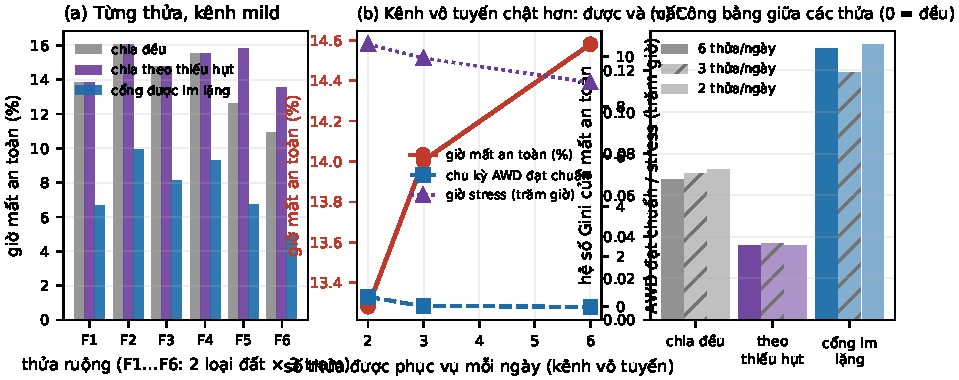
\includegraphics[width=0.70\textwidth]{fig6_multifield.pdf}
\caption{Hợp tác xã sáu thửa ở kênh severe, gồm (a) giờ mất an toàn theo từng thửa với ba luật phân bổ; (b) đánh đổi khi kênh vô tuyến chật hơn; (c) hệ số Gini của phân bố mất an toàn.}
\label{fig:htx}
\end{figure}

\section{Thảo luận}

\emph{Liên hệ chuẩn MRV.} Nhật ký lệnh (audit trail) của cổng, gồm lệnh, thời điểm, độ sâu, trạng thái đã tới ruộng hay bị giữ lại kèm lý do theo từng chu kỳ, chính là ``hồ sơ tưới tiêu \& rút nước thực tế'', bậc bằng chứng cao nhất trong thứ tự ưu tiên của QĐ 4801, ở độ phân giải giờ, thay cho ảnh chụp thủ công mà quy trình hiện đang yêu cầu. Bất biến hiệu chuẩn của cổng dùng đúng bộ máy khoảng tin cậy 95\% với $z=1{,}96$ mà Phụ lục A12 của QĐ 4801 quy định cho báo cáo độ không chắc chắn trong MRV; tính bảo thủ của $\sigma$ thể hiện ở bất biến I7 cũng cùng hướng với nguyên tắc bảo thủ tại Mục 9.3 của VM0051. Cần nói rõ giới hạn: hệ thống này \emph{không} lượng hóa phát thải khí mê-tan (CH$_4$) và khí nitơ oxit (N$_2$O), không thay thế bộ hệ số phát thải theo vụ do Viện Môi trường Nông nghiệp (IAE) xây dựng, và không thay khâu thẩm định của bên thứ ba. Nó là tầng ra quyết định sinh ra dữ liệu hoạt động (activity data) đạt cấp MRV chứ không phải một hệ MRV hoàn chỉnh. Ràng buộc vận hành của QĐ 4801, theo đó rút nước chỉ được coi là hiệu quả nếu ruộng không bị tưới lại trong ít nhất ba ngày, đã được mã hóa thành chỉ số đo chính của bài: mỗi chu kỳ chỉ được đếm là \emph{đạt chuẩn} khi pha khô kéo dài $\ge$72 giờ, và chính chỉ số này đã sinh ra ngưỡng $f_\sigma \le 0{,}025$ nêu ở Mục~\ref{sec:deploy}.

\emph{Vì sao WITHHELD là một đóng góp chứ không phải thất bại.} Mọi bộ lập lịch theo tuổi thông tin đều buộc phải phát một gói nào đó; ở đây im lặng có cấu trúc rõ ràng: khi bản sao số quá mờ ($\sigma \ge \sigma^{*}$) hoặc nguồn nước quá mặn đến mức không còn giờ nào đủ ngọt, hành động đúng duy nhất là không hành động và ghi lại lý do. Điều này khớp với thực tế vận hành ở ĐBSCL là chờ con nước, đồng thời cung cấp cho MRV một loại bản ghi mới là \emph{bằng chứng của việc không làm}, loại thông tin mà ảnh vệ tinh có tần suất chụp hai đến bốn ngày khó tái dựng được.

\emph{Limitations.} (i) Mô phỏng, chưa thực địa; N = 3 trạm; đất dùng tham số trung bình FAO-56. (ii) $\sigma$ hơi bảo thủ, thể hiện ở tỷ lệ bao phủ 0,99--1,00 của bất biến I7. (iii) T2 là nghiệm cận biên (myopic), còn lời giải quy hoạch động (DP) đầy đủ vẫn để ngỏ. (iv) Ràng buộc C2 là mô hình tình huống, không có số đo mặn thực địa nên không dùng cho bất kỳ kết luận tuân thủ nào. (v) Ước tính thiệt hại năng suất do mặn chỉ là phép dịch tuyến tính $-12\%$ cho mỗi dS$\cdot$m$^{-1}$~\cite{usdaP1837} và bị chặn ở 100\%, không phải một mô hình năng suất đầy đủ. (vi) Khảo sát công trình đi trước chỉ thực hiện ở mức tóm tắt và chưa quét được cơ sở dữ liệu thư mục DBLP nên chưa loại trừ hết các hội nghị trong khu vực. (vii) Về tranh cãi nông học: tài liệu của Bộ Nông nghiệp Hoa Kỳ (USDA) ghi nhận lúa mẫn cảm với mặn nhất ở giai đoạn mạ trong khi mẫn cảm với nhiệt lại đạt đỉnh ở giai đoạn trổ, tức hai đỉnh lệch pha nhau; chúng tôi nêu cả hai phía thay vì chọn một. (viii) Kết quả phụ thuộc năm khí hậu, xem Mục~\ref{sec:twoyears}.

\section{Kết luận}

Chúng tôi đã trình bày một cổng an toàn ràng buộc cơ hội, dùng bản sao số có khả năng trả lời câu hỏi phản thực để kiểm soát việc phát lệnh tưới trên kênh mất gói, kèm ngưỡng độ trung thực $\sigma^{*}=W/(2z_{1-\delta/2})$ giải thích khi nào im lặng là tối ưu. Trên 36\,480 lần mô phỏng với dữ liệu ERA5 thật tại ba trạm ở ĐBSCL qua hai năm khí hậu, cổng đề xuất không thua bất kỳ mốc cơ sở nào ở bất kỳ ô nào có ý nghĩa thống kê, thắng đậm trong điều kiện khan nước và hòa khi nước dư; gửi lại theo niềm tin giảm 23\% nước lãng phí do tưới đúp so với gửi lại mù; và trong mô hình tình huống mặn thì loại trừ hoàn toàn việc bơm mặn với giá phải trả đo được. Ba điều kiện áp dụng đã được lượng hóa chứ không mặc định: độ trung thực của bản sao số phải vượt ngưỡng $\sigma^{*}$ (để cổng không rỗng) và ngưỡng $f_\sigma \le 0{,}025$ (để chu kỳ AWD đủ 72 giờ theo QĐ 4801); độ phân giải lệnh của thiết bị chấp hành phải đạt mức 20\,mm (mức thô 35\,mm làm mất an toàn tăng từ 0,28\% lên 9,65\%); và lợi thế của cơ chế im lặng tắt dần khi nước dư, với điểm chéo đo được ở 320\,mm mỗi thửa. Mã nguồn, bảy bất biến, dữ liệu và toàn bộ kết quả đều tái lập được. Hướng tiếp theo gồm mở rộng T2 thành bài toán quy hoạch động đầy đủ, và hiệu chuẩn $\sigma$ bằng số đo mực nước thực địa khi có.

\section*{Dữ liệu và mã nguồn}
Toàn bộ mã nguồn, bảy bất biến, dữ liệu thời tiết kèm tệp xuất xứ, và 36\,480 dòng kết quả thô đứng sau mọi con số trong bài được công bố công khai tại \url{https://github.com/mxuanvan02/TwinGate} (giấy phép MIT). Tập lệnh \texttt{reproduce.sh} tái lập toàn bộ kết quả từ một bản sao sạch: tự tạo môi trường ảo, tải lại dữ liệu ERA5 qua giao diện lưu trữ công khai Open-Meteo, chạy các bộ kiểm thử rồi sinh lại mọi hình và bảng. Các văn bản chính sách của bên thứ ba (VM0051 của Verra, QĐ 4801/QĐ-BNNMT, QĐ 1490/QĐ-TTg) không được phân phối lại trong kho mã mà chỉ trích dẫn nguồn công khai.

\section*{Lời cảm ơn}
Nghiên cứu này được tài trợ bởi Đại học Huế trong khuôn khổ đề tài mã số DHH2025-19-07. Dữ liệu khí hậu lấy từ ERA5 thông qua giao diện lập trình ứng dụng thời tiết lịch sử của Open-Meteo. Khung vấn đề MRV được xây dựng từ các tài liệu công khai của Verra (VM0051 phiên bản 1.1), Bộ Nông nghiệp và Môi trường (QĐ 4801/QĐ-BNNMT) và Thủ tướng Chính phủ (QĐ 1490/QĐ-TTg).

\bibliography{refs}

\appendix
\section*{Phụ lục A. Khảo sát prior art tóm tắt}
Khảo sát trên OpenAlex giai đoạn 2015--2026 với 461 bản ghi, không có lỗi giao diện lập trình ứng dụng nào, được phân loại bằng biểu thức chính quy ở mức tóm tắt thành sáu nhóm: A bản sao số (64); B MRV và tín chỉ các-bon (22); C khí mê-tan ruộng lúa (93); D AWD và mực nước (45); E kênh mất gói và IoT (77); F chặn trên bất định và bảo đảm xác suất (2). Các giao A$\cap$B$\cap$C, A$\cap$B$\cap$C$\cap$D, A$\cap$B$\cap$C$\cap$D$\cap$E và A$\cap$B$\cap$C$\cap$D$\cap$E$\cap$F đều bằng 0. Các công trình gần nhất là bản sao số cho phục hồi rừng~\cite{sasaki2025}, trí tuệ nhân tạo kết hợp chuỗi khối cho thị trường các-bon~\cite{islam2025}, và bản sao số cho năng suất lúa (tiền bản thảo trên SSRN năm 2024, không liên quan MRV)~\cite{narayanan2024}. Hạn chế: khảo sát chỉ ở mức tóm tắt; chưa quét được DBLP nên chưa loại trừ các hội nghị khu vực gồm KSE, RIVF, ACIIDS và IUKM; dữ liệu quét lưu tại \texttt{gapscan\_MRV/} và \texttt{gapscan\_K1/}.

\section*{Phụ lục B. Bảng bất biến}
I1 ngân sách cứng (mức vượt tệ nhất 0,000\,mm trên 108 lần mô phỏng); I2 mỗi chu kỳ chỉ một quyết định; I3 độ sâu nước thực tới ruộng nằm trong $[20;60]$\,mm; I4 số lệnh tới ruộng không vượt số lệnh gửi và lượng nước lãng phí do tưới đúp không vượt lượng đã tưới; I5 không chính sách nào vượt Oracle quá 0,5 điểm phần trăm; I6 tắt tái neo dẫn tới 0 lệnh, tỷ lệ mất an toàn 57,82\% và RMSE bằng 0,000 do trùng khớp suy biến; I7 tỷ lệ bao phủ đạt 0,9906--1,0000 với $n{=}6480$ mẫu mỗi ô. Toàn bộ chạy tự động và trả về mã thoát 0.

\vspace{1em}
\hrule
\vspace{0.5em}

{\centering\bfseries A Digital-Twin Safety Gate for Irrigation Command Dispatch over Lossy Networks and Its Relevance to Emission MRV\par}
\vspace{0.8em}

\section*{Abstract}

The cost of measurement, reporting and verification (MRV) is the bottleneck for rice carbon credits in the Mekong Delta, and every credit-eligible water-management action passes through a control command sent over an unreliable wireless channel. We cast the problem as a networked control system: a safety gate uses a digital twin of the FAO-56 water balance to simulate each candidate command before transmission, releasing it only when the field is predicted to remain safe with sufficiently high probability, a chance constraint on irrigation scheduling. We prove that the twin has an accuracy threshold computed in closed form from the width of the agronomic safe zone: beyond it the gate cannot release any command and silence is optimal. Simulations on real ERA5 weather at three Delta stations show that the gate clearly reduces unsafe hours against every baseline when water is scarce; paired tests record no cell where the gate loses significantly. Credit-eligible alternate wetting-and-drying cycles appear only when the twin meets that threshold, a condition that more frequent sensing cannot remedy. In a tidal-salinity scenario model the gate excludes saline pumping entirely. The gate's command log is MRV-grade activity data under Decision 4801/QD-BNNMT; code and data are published at \url{https://github.com/mxuanvan02/TwinGate}.

\noindent\textbf{Keywords:} digital twin; networked control system; chance constraint; irrigation scheduling; MRV

\vspace{1em}
\hrule
\vspace{0.5em}

\section*{Thông tin tác giả}

\noindent
\textbf{Nguyễn Tương Tri}, Tiến sĩ\\
Trường Đại học Sư phạm, Đại học Huế, 34 Lê Lợi, TP Huế\\
Viện Đào tạo Mở và Công nghệ thông tin, Đại học Huế\\
Email: nguyentuongtri@dhsphue.edu.vn / ntuongtri@hueuni.edu.vn\\
Điện thoại: [PLACEHOLDER]\\
Tác giả liên hệ (corresponding author): Nguyễn Tương Tri\\[6pt]
{\small [Chữ ký tác giả: bản in ký + scan trước khi nộp]}

\end{document}
